% CVPR 2024 Paper Template; see https://github.com/cvpr-org/author-kit

\documentclass[10pt,twocolumn,letterpaper, pagenumbers]{article}

%%%%%%%%% PAPER TYPE  - PLEASE UPDATE FOR FINAL VERSION
\usepackage{cvpr}              % To produce the CAMERA-READY version
%\usepackage[review]{cvpr}      % To produce the REVIEW version
%\usepackage[pagenumbers]{cvpr} % To force page numbers, e.g. for an arXiv version

% Import additional packages in the preamble file, before hyperref
%
% --- inline annotations
%
\usepackage[dvipsnames]{xcolor}
\newcommand{\red}[1]{{\color{red}#1}}
\newcommand{\todo}[1]{{\color{red}#1}}
\newcommand{\TODO}[1]{\textbf{\color{red}[TODO: #1]}}
% --- disable by uncommenting  
% \renewcommand{\TODO}[1]{}
% \renewcommand{\todo}[1]{#1}



% It is strongly recommended to use hyperref, especially for the review version.
% hyperref with option pagebackref eases the reviewers' job.
% Please disable hyperref *only* if you encounter grave issues, 
% e.g. with the file validation for the camera-ready version.
%
% If you comment hyperref and then uncomment it, you should delete *.aux before re-running LaTeX.
% (Or just hit 'q' on the first LaTeX run, let it finish, and you should be clear).
\definecolor{cvprblue}{rgb}{0.21,0.49,0.74}
\usepackage[pagebackref,breaklinks,colorlinks,citecolor=cvprblue]{hyperref}

%%%%%%%%% PAPER ID  
\def\paperID{*****} % *** Enter the Paper ID here
\def\confName{EarthVision}
\def\confYear{2024}

%%%%%%%%% TITLE 
\title{Reevaluation of Foundation Models in \\"Geography-Aware Self-Supervised Learning”}

%%%%%%%%% AUTHORS - PLEASE UPDATE
\author{Hanna Lichtenberg\\
Technical University of Berlin\\
{\tt\small h.lichtenberg@campus.tu-berlin.de}
}

\begin{document}
\maketitle
\begin{abstract}
%The ABSTRACT is to be in fully justified italicized text, at the top of the left-hand column, below the author and affiliation information.
%Use the word ``Abstract'' as the title, in 12-point Times, boldface type, centered relative to the column, initially capitalized.
%The abstract is to be in 10-point, single-spaced type.
%Leave two blank lines after the Abstract, then begin the main text.
%Look at previous \confName~abstracts to get a feel for style and length.

Foundation models, trained on large datasets in a self-supervised manner, have become useful tools in artificial intelligence, especially in domains with abundant unlabeled data but scarce labeled data, such as remote sensing. This study re-evaluates the MoCo-v2 framework and compares it with a geography-aware contrastive learning approach introduced by Ayush et al. in the paper "Geography-Aware Self-Supervised Learning" \cite{geoAwareSelfSuper}. This approach leverages spatio-temporal structures in remote-sensing data and combines it with a geo-location classification pre-text task. I used the BigEarthNet dataset to evaulate the expressivness of the models' feature representations in several experiments. The experiments demonstrate that integrating metadata, particularly geo-location information, into foundation models is likely to improve performance in multi-label classification tasks. 

\end{abstract}    
\section{Introduction}
\label{sec:intro}

Foundation models represent a significant advancement in the field of artificial intelligence and machine learning due to their ability to serve as a versatile base for a wide range of tasks and applications. The models are pretrained on large, diverse datasets in a self supervised manner, allowing them to learn general features and patterns. This pretraining stage enables the models to perform well on various downstream tasks with minimal additional fine-tuning, reducing the need for extensive labeled datasets for each specific task. \cite{foundationModels} \\
In the context of Earth observation, unlabeled data is often abundant, while labeled data is scarce, particularly in geolocated datasets such as those used in remote sensing \cite{geoAwareSelfSuper}. Foundation models are highly valuable in this field because they can be pretrained without the need for labels, using un-supervised or self-supervised learning techniques. \\
When evaluating a foundation model, the quality of the learned features is important. There are two main types of evaluation: intrinsic and extrinsic. Intrinsic evaluation assesses the model based solely on the learned features, focusing on their expressiveness and quality. In contrast, extrinsic evaluation measures the model's performance on an external downstream task. \cite{foundationModels} \\
This paper analyses the application of selected foundation models on the BigEarthNet dataset \cite{bigEartNetMM} using both types of evaluation. The external downstream task is multi-label classification. Fig. \ref{fig:setup} illustrates the evaluation setup.

\begin{figure}[t]
  \centering
   %\fbox{\rule{0pt}{1.5in} \rule{0.9\linewidth}{0pt}}
   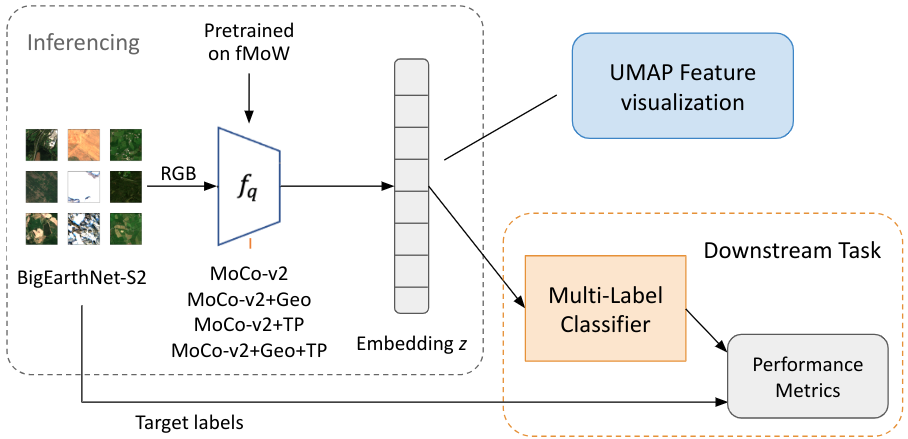
\includegraphics[width=\linewidth]{figures/ExperimentSetup.png}
   \caption{Illustration of the evaluation experiments on the BigEarthNet dataset: The query encoder of the examined MoCo-v2 based foundation models is used to extract featuress $z$, which are then evaluated through UMAP feature visualization and the performance of a classifier on the multi-label classification downstream task.}
   \label{fig:setup}
\end{figure}


\section{Related Work}
\label{sec:formatting}

\begin{figure*}
\begin{minipage}[t]{0.52\linewidth}
    \centering
    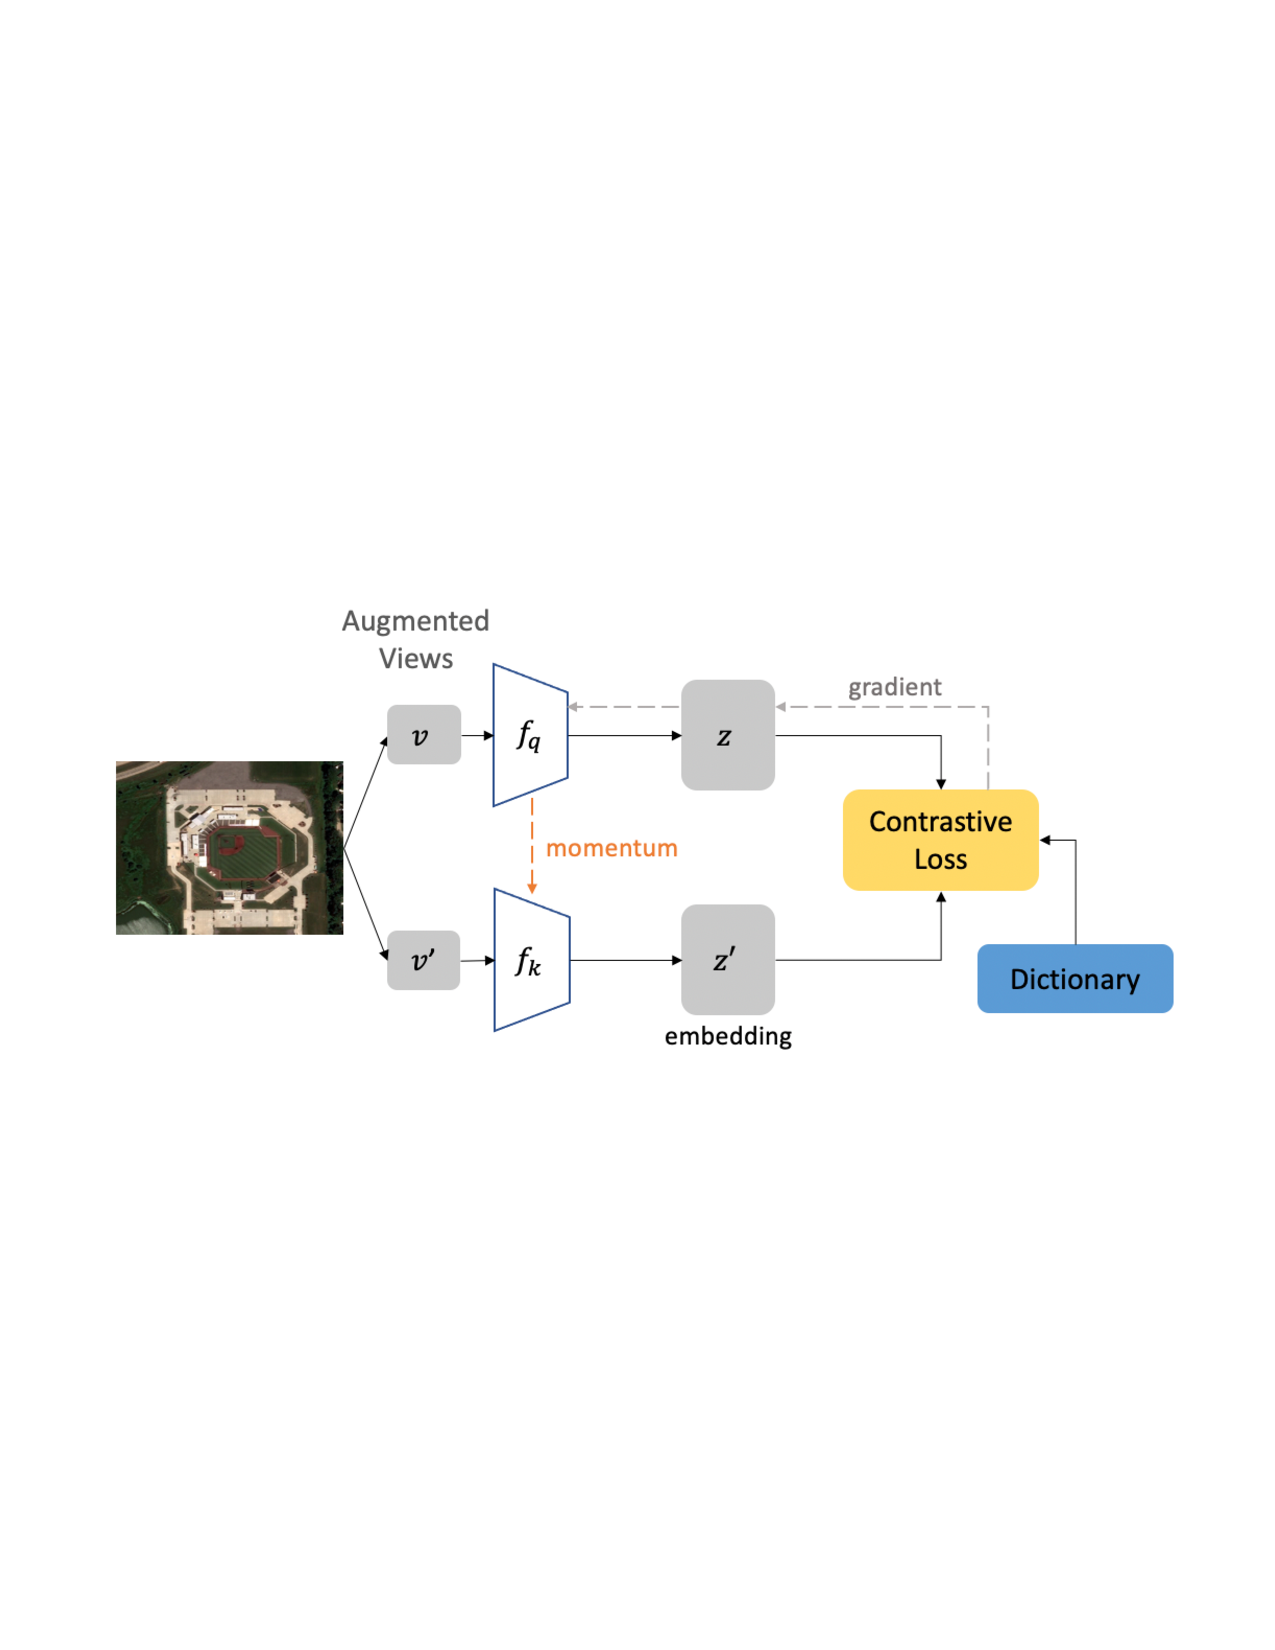
\includegraphics[width=\linewidth]{figures/ap1.pdf}
    \caption{Schematic overview of the original MoCo-v2 framework \\(figure by \cite{geoAwareSelfSuper}).}
    \label{fig:Moco}
\end{minipage}
\hfill
\begin{minipage}[t]{0.44\linewidth}
    \centering
    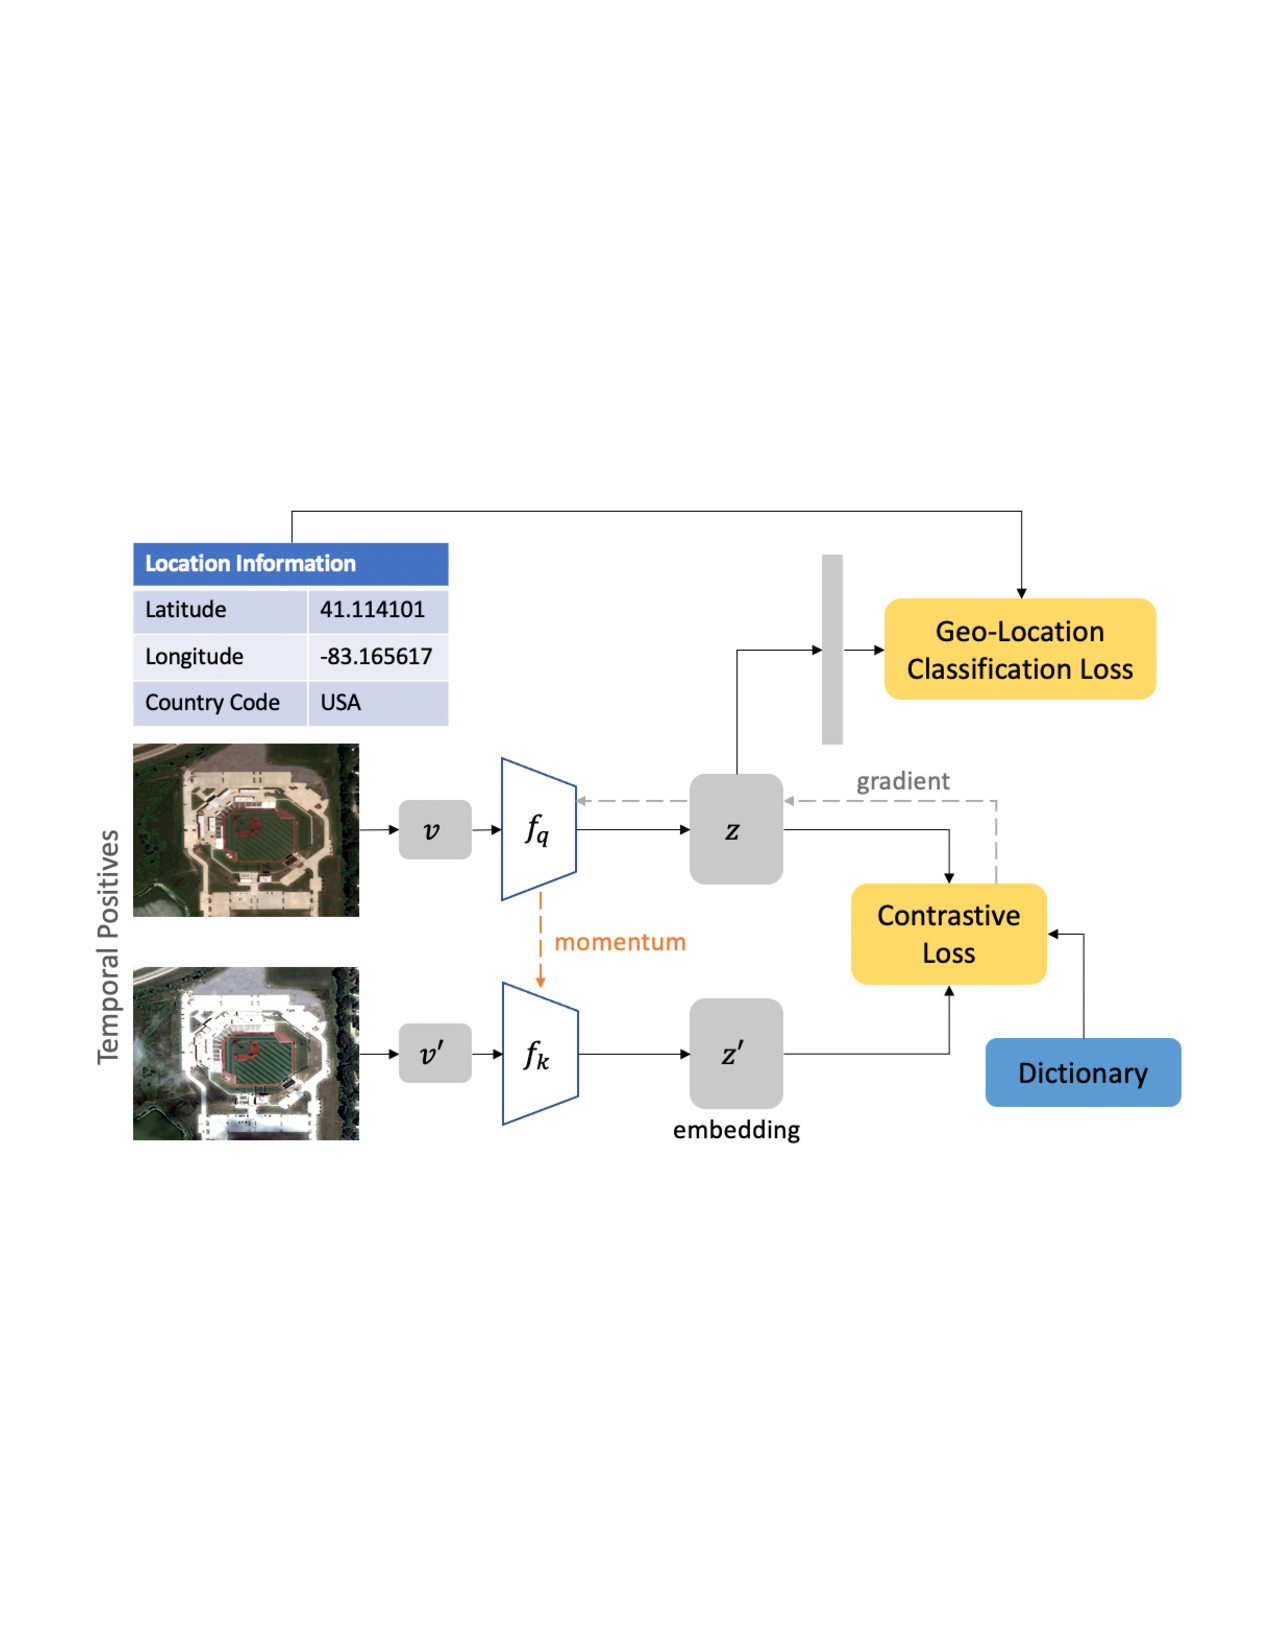
\includegraphics[width=\linewidth]{figures/ap2.pdf}
    \caption{Geography-aware contrastive learning approach (figure by \cite{geoAwareSelfSuper}).}
    \label{fig:geography_aware}
\end{minipage}
\end{figure*}

Self-supervised models for satellite data face several challenges due to the unique characteristics of the data, such as the temporal dimension, their large-scale nature and the availability of data from various complementary sensors \cite{presto}. These factors complicate the modeling process, requiring the use of sophisticated foundation model techniques. \\
Most state-of-the-art models are based on transformer networks, often in combination with masked autoencoders. Transformer models are designed to handle sequential data, weighing the importance of different elements within the sequence \cite{transformer}. This capability makes them particularly well-suited for the temporal dimension of satellite data, where capturing long-range dependencies and relationships is crucial. \\
In a masked autoencoder parts of the input data are hidden during training, and the model learns to reconstruct the missing parts from the remaining visible parts \cite{maskedAutoEncoder}. This approach is particularly useful for learning robust feature representations and dealing with incomplete data. Masked autoencoders benefit from the powerful feature extraction capabilities of transformers. By using a transformer as the backbone, the model can effectively handle sequential and high-dimensional data. Examples are SatMAE \cite{SatMAE}, Presto \cite{presto} and RVSA \cite{rvsa}. These models use techniques like temporal embeddings, masking image patches across time and associated metadata. RVSA introduces a lage-scale vision transformer which replaces the full attention in transformers with a new rotated varied-size window attention to reduce computational cost and memory footprint. \\
Other approaches train diffusion models like DiffusionSat \cite{DiffSat} and PreDiff  \cite{prediff}. A diffusion model is a type of generative model that gradually transforms noise into a target data distribution through a series of iterative steps, often used for data generation \cite{diffusion}. DiffusionSat conditions the model on metadata such as geolocation to generate realistic samples, while PreDiff introduces a two-stage pipeline for probabilistic spatiotemporal forecasting. \\
There are other self-supervised learning methods used in foundation models for Earth observation that have received less attention in the literature. One such method is contrastive learning which trains models by distinguishing between similar (positive pairs) and dissimilar data pairs. This approach encourages closeness of representations of images that are likely to be semantically similar. \cite{geoAwareSelfSuper} \\
In this paper the quality of the contrastive learning foundation models introduced by K. Ayush et al. \cite{geoAwareSelfSuper} are exaulated on a remote sensing dataset.


\section{Geography-Aware Self-Supervised Learning}
\label{sec:methodology}

This section provides a brief introduction to the geography-aware contrastive learning approach presented in \cite{geoAwareSelfSuper}. Initially, they evaluated the state-of-the-art self-supervised contrastive learning method, MoCo-v2 \cite{mocoV2}, on remote sensing datasets such as the Functional Map of the World (fMoW) image classification benchmark \cite{fmow}. The evaluation revealed a performance gap between the self-supervised learning and supervised learning using labels. \\
To bridge this gab they introduced geography-aware contrastive learning to leverage the spatio-temporal structure of remote sensing data. Unlike contrastive learning for traditional computer vision images where different views of the same image serve as a positive pair as in MoCo-v2, they propose to use temporal positive pairs from spatially aligned images over time. By doing so, the representations tent to be invariant to subtle variations over time, e.g. to seasons or weather. \\
They further designed an unsupervised learning method that uses geo-location information as a pre-text task. The task is to predict where in the world an image comes from. Models performing well in that task should be able to identify visual cues that are transferable to other downstream tasks. Both methods can be integrated into a single geography-aware contrastive learning objective. \\


\begin{figure}[t]
  \centering
   %\fbox{\rule{0pt}{1.5in} \rule{0.9\linewidth}{0pt}}
   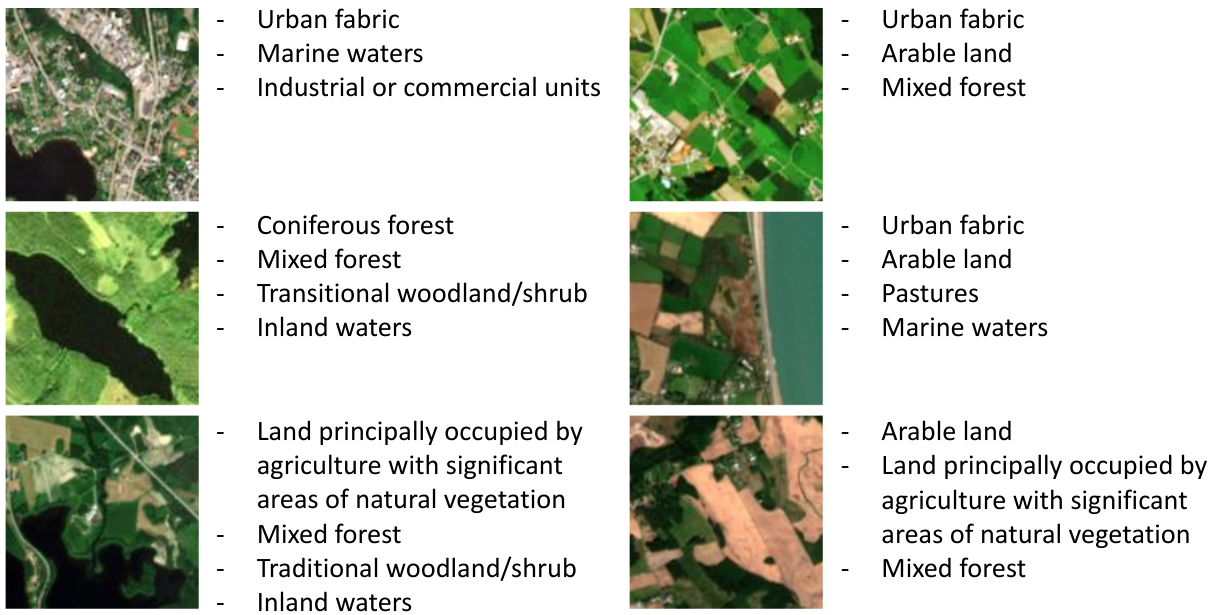
\includegraphics[width=\linewidth]{figures/BigEarthNet.png}
   \caption{Examples of Sentinel-2 images and their multi-lables in the BigEarthNet-MM dataset (adapted from \cite{BigEarthNetImg}).}
   \label{fig:BigEarth}
\end{figure}

\subsection{Contrastive Learning with temporal positive pairs}

The authors consider a geo-tagged visual dataset $\{((x_i^1, ..., x_i^{T_i}), $lat$_i, $lon$_i)\}_{i=1}^N$ where the $i$th datapoint consists of a sequence of images $(x_i^1, ..., x_i^{T_i})$ at a shared loaction with latitude (lat) and longituda (lon) over time $t_i = 1, ..., T_i$. The fMoW dataset fits these criteria. \\
Contrastive methods define a mapping $f_q: x_i^t \mapsto z_i^t \in \mathbb{R}^d$ from pixels $x_i^t$ to latent representations $z_i^t$. Models should learn representations by pulling positive images pairs from the same instance closer in latent space while pushing negative pairs from different instantes further away. \\
The Moco-v2 and the geography-aware contrastive learning framework are shown in Fig. \ref{fig:Moco} and Fig. \ref{fig:geography_aware}.
The objective is defined as follows \cite{geoAwareSelfSuper}:
\begin{equation}
    \label{eq:contrastive_loss}
    L_z = - \log\frac{\exp(z\cdot z'/\lambda)}{\exp(z\cdot z'/\lambda) + \sum_{j=1}^N \exp(z\cdot k_j/\lambda)},
\end{equation}
where $z$ and $z'$ are the encoded representations of a positive data pair $v$ and $v'$. $N$ is the number of negative samples, $\{k_j\}_{j=1}^N$ are the encoded negative pairs and $\lambda\in\mathbb{R}^+$ is the temperature hyperparameter. The similarity of the representations is measured by the dot product. \\
In MoCo-v2 the positive pair $v$ and $v'$ are two augmented views of an image $x_i^t$. Ayush et al. \cite{geoAwareSelfSuper} create positive pairs from a sequence of images $(x_i^1, ..., x_i^{T_i})$ by selecting a random image $x_i^{t_2}$ to pair with a given image $x_i^{t_1}$. They then apply pertubations like random color jittering to the spatially aligned image pair $x_i^{t_1}$ and $x_i^{t_2}$ resulting in the \textit{temporal positive pair} $v$ and $v'$. For training $v$ and $v'$ are passed through query and key encoders, $f_q$ and $f_k$, respectively.

\subsection{Combining Geo-location Classification and Contrastive Learning}

The geo-location classification pre-text task aims to further improve the quality of the representations. Ayush et al. \cite{geoAwareSelfSuper} cluster the images in the dataset using the coordinates $($lat$_i,$ lon$_i)$. They construct $K$ clusters with a clustering method and assign the areas a categorical geo-label $c_i\in\{1, ..., K\}$. By doing so, they are able to train a geo-location predictor CNN using cross entropy loss. \\
To combine both approaches they use the latent features $z_i^t$ from the contrastive learning query encoder as the input to the geo-location prediction network as shown in Fig. \ref{fig:geography_aware}. They perform joint learning by defining the final loss as the linear combination of the contrastive learning loss $L_z$ in Eq. \ref{eq:contrastive_loss} and the negative cross-entropy loss $L_g$ of the geo-location network with coefficients $\alpha$ and $\beta$: $L_f = \alpha L_z + \beta L_g$. \\
By minimizing $L_f$ they learn representations to jointly maximize agreement between spatio-temporal positive pairs, minimize agreement between negative pairs and predict the geo-label of the images from the positive pairs.

\begin{figure*}[t]
  \centering
   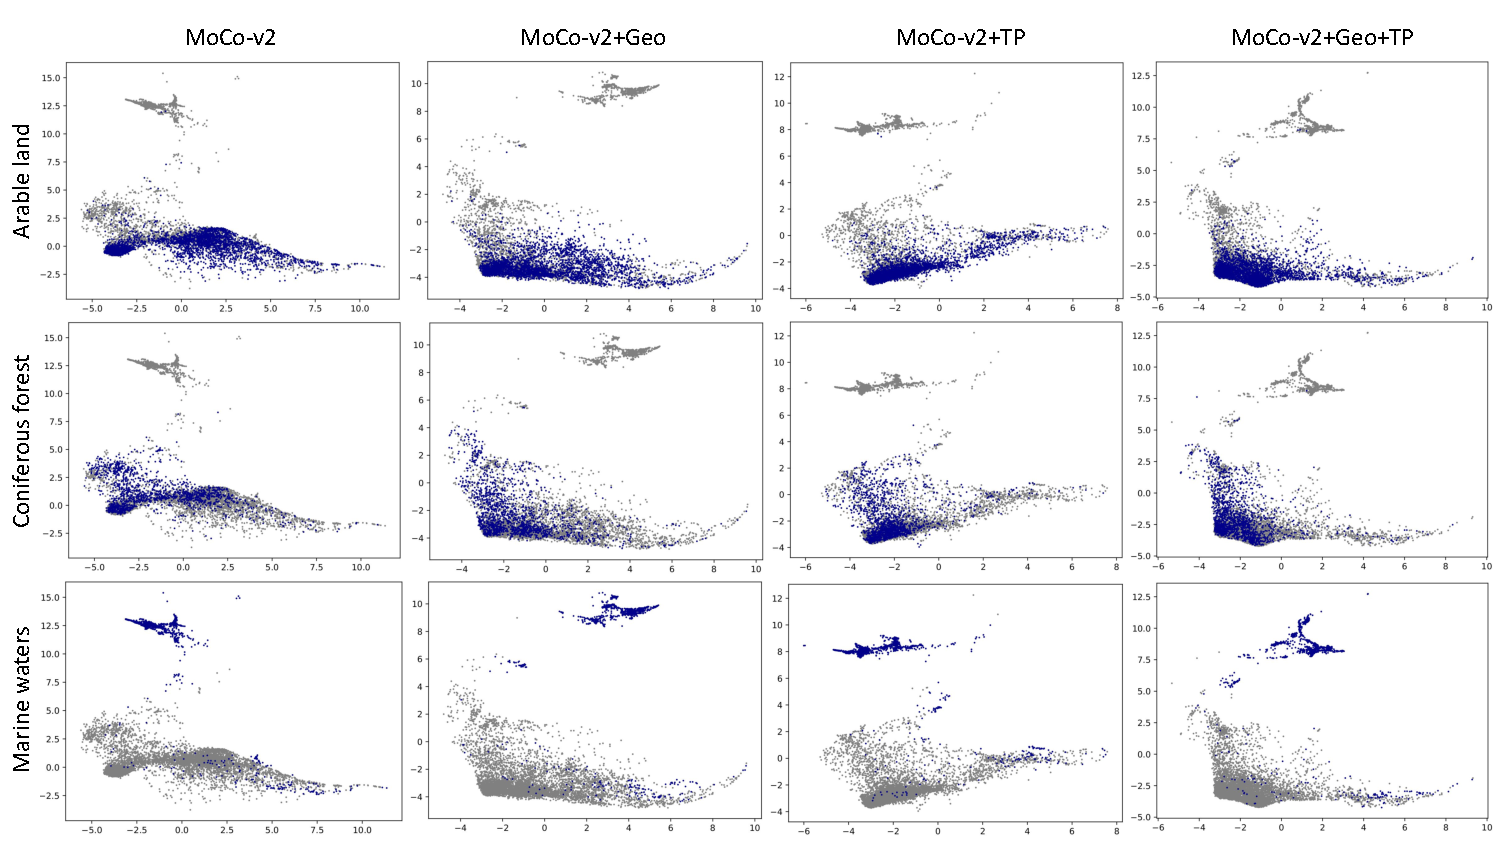
\includegraphics[width=\linewidth]{figures/UMAPVisualization.pdf}
   \caption{UMAP feature visualization of the BigEarthNet test data's feature vectors of the four foundation models. Data points corresponding to the labels \textit{arable land}, \textit{coniferous forest}, and \textit{marine waters} are highlighted in blue.}
   \label{fig:umap}
\end{figure*}
\section{Experiments}

For the following experiments, the Sentinel-2 bands of the BigEarthNet-MM dataset \cite{bigEartNetMM} are used. The latent representations of this data are examined intrinsically using UMAP feature visualization to determine if the embeddings naturally group similar items together and separate dissimilar ones. Extrinsic evaluation assesses the model's performance on an external downstream task, which depends on both the foundation model and the adaptation mechanism \cite{foundationModels}. In the performed extrinsic experiments, classifying the BigEarthNet data is chosen as the downstream task. Linear probing and classification with a simple Multiple Layer Perceptron are examined. The model's performance is analysed without retraining it on the classification data to only evaluate the information stored in the feature vectors. \\
The authors of the contrastive learning model \cite{geoAwareSelfSuper} provide their code as well as weights for four models: the original MoCo-v2 model, the MoCo-v2 model additionally trained on the geo-location pre-text task (MoCo-v2+Geo), the MoCo-v2 model trained with temporal positive pairs (MoCo-v2+TP), and the MoCo-v2 model trained on the pretext task in combination with temporal positive pairs (MoCo-v2+Geo+TP). They use the ResNet-50 \cite{resnet} architecture to parameterize the query and key encoders $f_q$ and $f_k$ for each model. For inferencing only the query encoder ist used. The weights are pre-trained on the fMoW \cite{fmow} dataset. The evaluation setup is illustrated in Fig. \ref{fig:setup}.

\subsection{Data - BigEarthNet-MM}

The BigEarthMet-MM benchmark dataset by Sumbul et al. \cite{bigEartNetMM} is designed for multi-modal and multi-label remote sensing applications. It consists of satellite images, i.e.  590,326 pairs of Sentinel-1 and Sentinel-2 image patches, acquired over 10 different European countries, each of which $120\times120$ pixels. The patches are annotated with multi-labels provided by the CORINE Land Cover (CLC) map of 2018, such as \textit{Broad-leaved forest} and \textit{Beaches, dunes, sands}. In total, the image patches are representative of 43 CLC classes. Sumbul et al. \cite{bigEartNetMM} also created a new class-nomenclature by modifying the CLC multi-labels resulting in 19 classes. CLC classes that are not feasible to be identified by only using single-date BigEarthNet-MM images are removed and others are grouped into new classes. \\
For the evaluation of the contrastive learning foundation model, 19 classes were chosen. Since the foundation model is designed to accept inputs of one modality at a time, only the Sentinel-2 images are used (BigEarthNet-S2). Examples are shown in Fig. \ref{fig:BigEarth}. \\
During the self-supervised pretraining of the foundation model, the fMoW data is normalized using z-score normalization. The fMoW images consist of RGB channels, which fit the ResNet-50 architecture designed for data with three input color channels. The spectral bands of the BigEarthNet-S2 dataset also include the visible spectrum bands: Red (B04), Green (B03), and Blue (B02). By selecting these bands and normalizing the data, the BigEarthNet-S2 images are prepared similarly to the fMoW images, providing a solid basis for meaningful inference results.

\subsection{UMAP Feature Visualization}
UMAP (Uniform Manifold Approximation and Projection) is a manifold learning technique for dimensionality reduction by McInnes et al. \cite{umap}. It visualizes high-dimensional data in a low-dimensional space while preserving local and global structures of the data. This makes it particularly useful for visualizing complex datasets such as feature embeddings. The technique is based in Riemannian geometry and algebraic topology. \\
By transforming high-dimensional data into a 2D or 3D space, UMAP allows for the visualization of the distribution of embeddings. Given that the BigEarthNet-S2 dataset provides multi-class labels, this technique makes it possible to observe if embeddings of images within the same class cluster together, indicating low distances between them. Since images of the same class share many similar features, their embeddings should ideally be close to each other. \\
The embedding layer of the contrastive learning models is the final layer, allowing the outputs of the inferencing to be directly interpreted as latent feature representations. The feature vectors extracted by the provided models have a size of 128. For the visual evaluation these vectors are transformed into a 2D space. \\
Results for the categories \textit{arable land}, \textit{coniferous forest} and \textit{marine waters} are shown in Fig. \ref{fig:umap}. Feature vectors from the BigEarthNet-S2 test dataset are used here. In all four models, data points belonging to the \textit{marine waters} category (blue) form a distinct cluster, significantly separated from other points (grey). For most other categories, such as \textit{arable land} and \textit{coniferous forest}, there are only minor distribution shifts between the points of a given category and the other data points. These observations are consistent across all four models. Detailed UMAP visualizations, separated by each of the 19 classes, can be found in the supplementary material. This visual evaluation does not reveal performance differences between the four contrastive learning models. However, the test demonstrates that the feature embeddings retain some semantic information from the input images.

\subsection{Classification Downstream Task}
\label{sec:classification}
%In this section, the foundation models' performance is evaluated based on their ability to complete the BigEarthNet-S2 multi-label classification downstream tasks. 
Most of the existing deep learning based methods assume that training images are annotated by single-labels, however remote sensing images typically contain multiple classes and thus
can simultaneously be associated with multi-labels \cite{benchmark}. The following tests intent to show how well the models' learned representations can be transferred and utilized in such a real-world remote sensing scenario: the BigEarthNet-S2 multi-label classification tasks.

\begin{table*}[h]
\centering
\begin{tabular}{c|cccc|cccc|c}
& \multicolumn{4}{|c|}{\textbf{Linear probing}} & \multicolumn{4}{|c|}{\textbf{MLP}} & \textbf{Baseline} \\
& MoCo-v2 & +Geo & +TP & +Geo+TP & MoCo-v2 & +Geo & +TP & +Geo+TP & K-Branch CNN \\ \hline
$R_{macr}$ & 0.239 & \textbf{0.241} & \textbf{0.241} & 0.224 & 0.394 & \textbf{0.417} & 0.395 & 0.382 & \textit{\textbf{0.468}} \\
$F^2_{macr}$ & 0.260 & \textbf{0.267} & 0.265 & 0.245 & 0.424 & \textbf{0.448} & 0.426 & 0.413 & \textit{\textbf{0.446}} \\
$F^2_{micr}$ & \textbf{0.381} & 0.360 & 0.367 & 0.349 & 0.555 & \textbf{0.570} & 0.546 & 0.538 & \textit{\textbf{0.610}} \\
$HL$ & \textbf{0.115} & 0.117 & \textbf{0.115} & 0.119 & 0.091 & \textbf{0.090} & 0.093 & 0.095 & \textit{\textbf{0.041}} \\
$OE$ & \textbf{0.311}& 0.344 & 0.327 & 0.363 & 0.177 & \textbf{0.175} & 0.181 & 0.194 & \textit{\textbf{0.063}} \\
\end{tabular}
\caption{Multi-label classification results of the experiments in section \ref{sec:classification}. The linear probing and MLP classifiers are trained on the foundation models' embedding outputs for the 19-class BigEarthNet-S2 task, while the baseline model results pertain to the 43-class task.}
\label{tab:classification}
\end{table*}

\subsubsection{Performance Metrics}
To evaluate any multi-label classification approach it is necessary to analyse more than only the number of correct predictions. Therefore, several performance metrics are used to present the results of the multi-label experiments: Recall (R), F2-Score (F2), Hamming loss (HL) and One error (OE).  \\
There are different ways to calculate the classification based metrics recall and F2-Score. Macro averaging gives equal importance to each class by first computing the metrics per class and then averaging the class results. Micro averaging computes the metrics globally by treating each individual prediction as an atomic unit. \cite{benchmark} \\
During the experiments of these sections the recall is calculated with macro averaging and for the F2-Score both, micro and macro averaging, are reported. The following calculatioins originate from Sumbul et al. \cite{benchmark}. \\
Let $TP_{ij}$, $FP_{ij}$, $FN_{ij}$ and $FP_{ij}$ indicate the conditions of true positive, false positive, false negative and true negative for the $i^{th}$ sample and $j^{th}$ class label ($l_j$), where exactly one is true, value $1$, and the other three take $0$. The recall with macro averaging is expressed as follows: 
\begin{equation}
    R_{macr}=\frac{1}{S}\sum_{j=1}^S \frac{\sum_{i=1}^M TP_{ij}}{\sum_{i=1}^M TP_{ij}+FN_{ij}},
\end{equation}
where $S$ is the number of classes and $M$ the number of samples. The F2-Score is the weighted harmonic mean of the metrics precison and recall. It is defined as follows:
\begin{equation}
    F_{macr}^2 = \frac{1}{S}\sum_{j=1}^S \frac{\sum_{i=1}^M 5TP_{ij}}{\sum_{i=1}^M 5TP_{ij}+4FN_{ij} + FP_{ij}},
\end{equation}
\begin{equation}
    F_{micr}^2 = \frac{\sum_{i=1}^M\sum_{j=1}^S 5TP_{ij}}{\sum_{i=1}^M\sum_{j=1}^S 5TP_{ij}+4FN_{ij} + FP_{ij}}.
\end{equation}
The Hamming loss is the average Hamming distance
between the ground truth labels $y_i^*$ and predicted multilabels $y_i$:
\begin{equation}
    HL = \frac{1}{M}\sum_{i=1}^M\frac{1}{S}\sum_{j=1}^S [l_j\in y_i \oplus l_j \in y_i^*].
\end{equation}
Here $\oplus$ is the XOR logical operation. \\
The one error (OE) is a ranking-based metric which means it is defined with respect to the ranking of the $j^{th}$ label in the class probabilities output for the $i_{th}$ sample. The rank is defined as $rank_{ij}=|k:P(l_k|x_i)\geq P(l_j|x_i)|$. The rate of samples whose predicted label having the highest ranking is not in the ground truth label is expressed in the one error metric, defined as follows:
\begin{equation}
    OE = \frac{1}{M}\sum_{i=1}^M[\{\text{argmax}_j rank_{ij}\not\in y_i].
\end{equation}

\subsubsection{Linear Probing}
An effective method to utilize the features produced by a foundation model for training a classifier is linear probing. It involves fixing the weights of the foundation model and training a simple, one-layer model on top of it \cite{linProb}. This model, known as the linear head, takes the features as input and outputs the predicted labels. During training, only the linear head is optimized. It is well-established that fine-tuning the entire model after this step typically leads to a performance increase, as this is a successful transfer learning technique \cite{linProb}. However, due to limited computational resources, the experiments in this section do not include fine-tuning the whole model and the foundation model's weights remain unchanged. \\
The linear probing layer used in this experiment has 19 output units, each representing a class, with sigmoid activations to address the multi-label task. The layer is trained for 20 epochs on the feature vectors from the BigEarthNet-S2 train dataset, using binary cross-entropy loss and the Adam optimizer with a learning rate of $0.01$. The model weights from the epoch with the lowest validation loss are chosen for the final performance evaluation on the test data. \\
The left side of Tab. \ref{tab:classification} shows the results for the four foundation models. All models exhibit relatively poor performance in terms of the metrics. Surprisingly, there are only minor differences between the original MoCo-v2 approach and the MoCo-v2 models trained with geography-aware self-supervised learning. The model combining temporal positive pairs and geo-location classification performs even worse than the original MoCo-v2. \\
The overall lack of performance, with the best $F_{macr}^2$ being only $0.267$, is expected since linear probing can only model a linear function between the foundation models' embeddings and the class labels. However, the results indicate that the embeddings contain features of the Sentinel-2 images that are useful for classification, as they perform significantly better than random guessing\footnote{The class distribution in the multi-label task is highly imbalanced, with each image belonging to only a few of the 19 classes. Consequently, random guessing results in a very high number of false positives, causing the F2 score to be approximately zero.}.  

\subsubsection{Multiple Layer Perceptron (MLP)}

\begin{figure}[t]
  \centering
   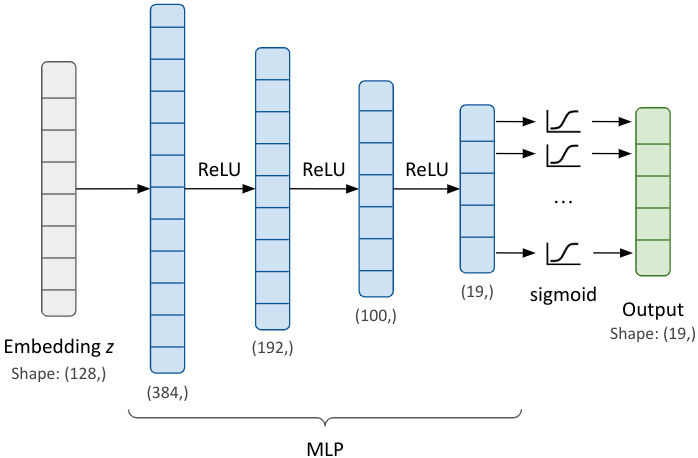
\includegraphics[width=\linewidth]{figures/mlp.png}
   \caption{Multi-label classification with the MLP.}
   \label{fig:mlp}
\end{figure}

While linear probing offers a straightforward approach, its limited approximation capabilities hinder its ability to capture complex relationships between the embeddings and class labels. In this experiment, a multi-layer perceptron (MLP) is used as classifier on top of the foundation model because of its enhanced approximation capabilities. By stacking multiple layers, the MLP can model complex patterns within the data, potentially leading to improved results. \\
The utilized a MLP consists of four layers, as illustrated in Fig. \ref{fig:mlp}. The classifier is trained using cross-entropy loss and the Adam optimizer with a learning rate of 0.001. To enhance performance, the learning rate is reduced when the validation loss stagnates. \\
Table \ref{tab:classification} shows the results in comparison with the linear probing. Further, results of a benchamrk classifier model for the BigEarthNet-S2 dataset with 43 classes are provided. As expected, the MLP classifier achieves significantly better results than linear probing. Among the foundation models, the MoCo-v2 model additionally trained on the geo-location classification pretext task outperforms the others. However, contrastive learning with temporal positive pairs does not lead to a performance increase in comparison with the original MoCo-v2. This pretraining approach is not advantageous for this specific multi-label classification downstream task, although previous work by Ayush et al. \cite{geoAwareSelfSuper} reported performance gains in various other downstream tasks such as image segmentation and object detection. \\
The baseline model - the K-Branch CNN - introduced by Sumbul et al. \cite{benchmark}, is specifically designed for multi-label classification of high-dimensional remote sensing images. It is trained directly on the BigEarthNet-S2 images without using a foundation model. This approach considers the complex spatial and spectral content of image local areas by defining spatial resolution-specific CNN branches followed by a multi-attention strategy to handle the importance scores of different local areas of each image. \\ 
Despite the K-Branch CNN's classification task involving all 43 classes, compared to the simpler 19-label classification of the foundation models, it still outperforms the four examined contrastive learning models.
However, given that the K-Branch CNN is fully optimized for the BigEarthNet-S2 data and the MLP only uses small feature embeddings of size 128, optimized for a different dataset (fMoW), the MLP results are impressive. The foundation models appear to generalize well, retaining the most useful information from the $120\times120$ Sentinel-2 images within an embedding vector of only 128 dimensions.  \\

\subsection{Discussion}

A significant limitation of the current experiments is the absence of complete transfer learning. Transfer learning typically involves fine-tuning the pre-trained model on the specific downstream task. This fine-tuning step was skipped in the experiments due to lack of computational ressources. Introducing a retraining phase for the foundation models' weights with a small learning rate could potentially lead to substantial performance improvements. \\
This shows further that the evaluation results are highly dependent on the adaptation mechanism and amount of optimization used. The performance improved significatly when using an MLP instead of linear probing which makes it difficult to evaluate the quality of a foundation model. This is a common downside of extrinsic evaluation \cite{foundationModels}. \\
The BigEarthNet dataset is large, offering a lot of test data for meaningful evaluation and making it sufficiently robust to train large models like the K-Branch CNN from scratch. This makes it difficult for foundation models to outperform the K-Branch CNN. The power of foundation models is more evident when dealing with smaller datasets, where transfer learning can provide significant better results with less overfitting compared to models trained from scratch.
\section{Conclusion}

My study demonstrates that integrating the metadata associated with remote-sensing data into contrastive learning foundation models improves their performance on the BigEarthNet Sentinel-2 dataset. The MLP classifier on top of the MoCo-v2 model pre-trained on the additional geo-location classification task achieves the best results. This indicates that creating foundation model architectures that are specifically adapted to the unique characteristics of remote sensing data can be very beneficial. \\ 
However, a limitation of the experiments is the absence of fine-tuning foundation models. A retraining phase on the BigEarthNet data could greatly improve the results. Also, the evaluation results depend a lot on the adaptation method, as shown by the huge improvement when using an MLP instead of linear probing.

{
    \small
    \bibliographystyle{ieeenat_fullname}
    \bibliography{main}
}

\clearpage
%\setcounter{page}{1}

\maketitlesupplementary

%\title{Reevaluation of Foundation Models in \\"Geography-Aware Self-Supervised Learning”}{Supplementary Material}
\section*{UMAP Feature Visualization} 

\vspace{10pt}
\begin{minipage}{\textwidth}
    The following figures visualize the UMAP features of the BigEarthNet-S2 test data's feature vectors extracted by the four re-evaluated foundation models.  The feature vectors that correspond to the specified class are shown in blue. This visualization is provided for each of the 19 labels. \\
\end{minipage}

\begin{figure}[htbp]
  \centering
   \begin{minipage}{\textwidth}
   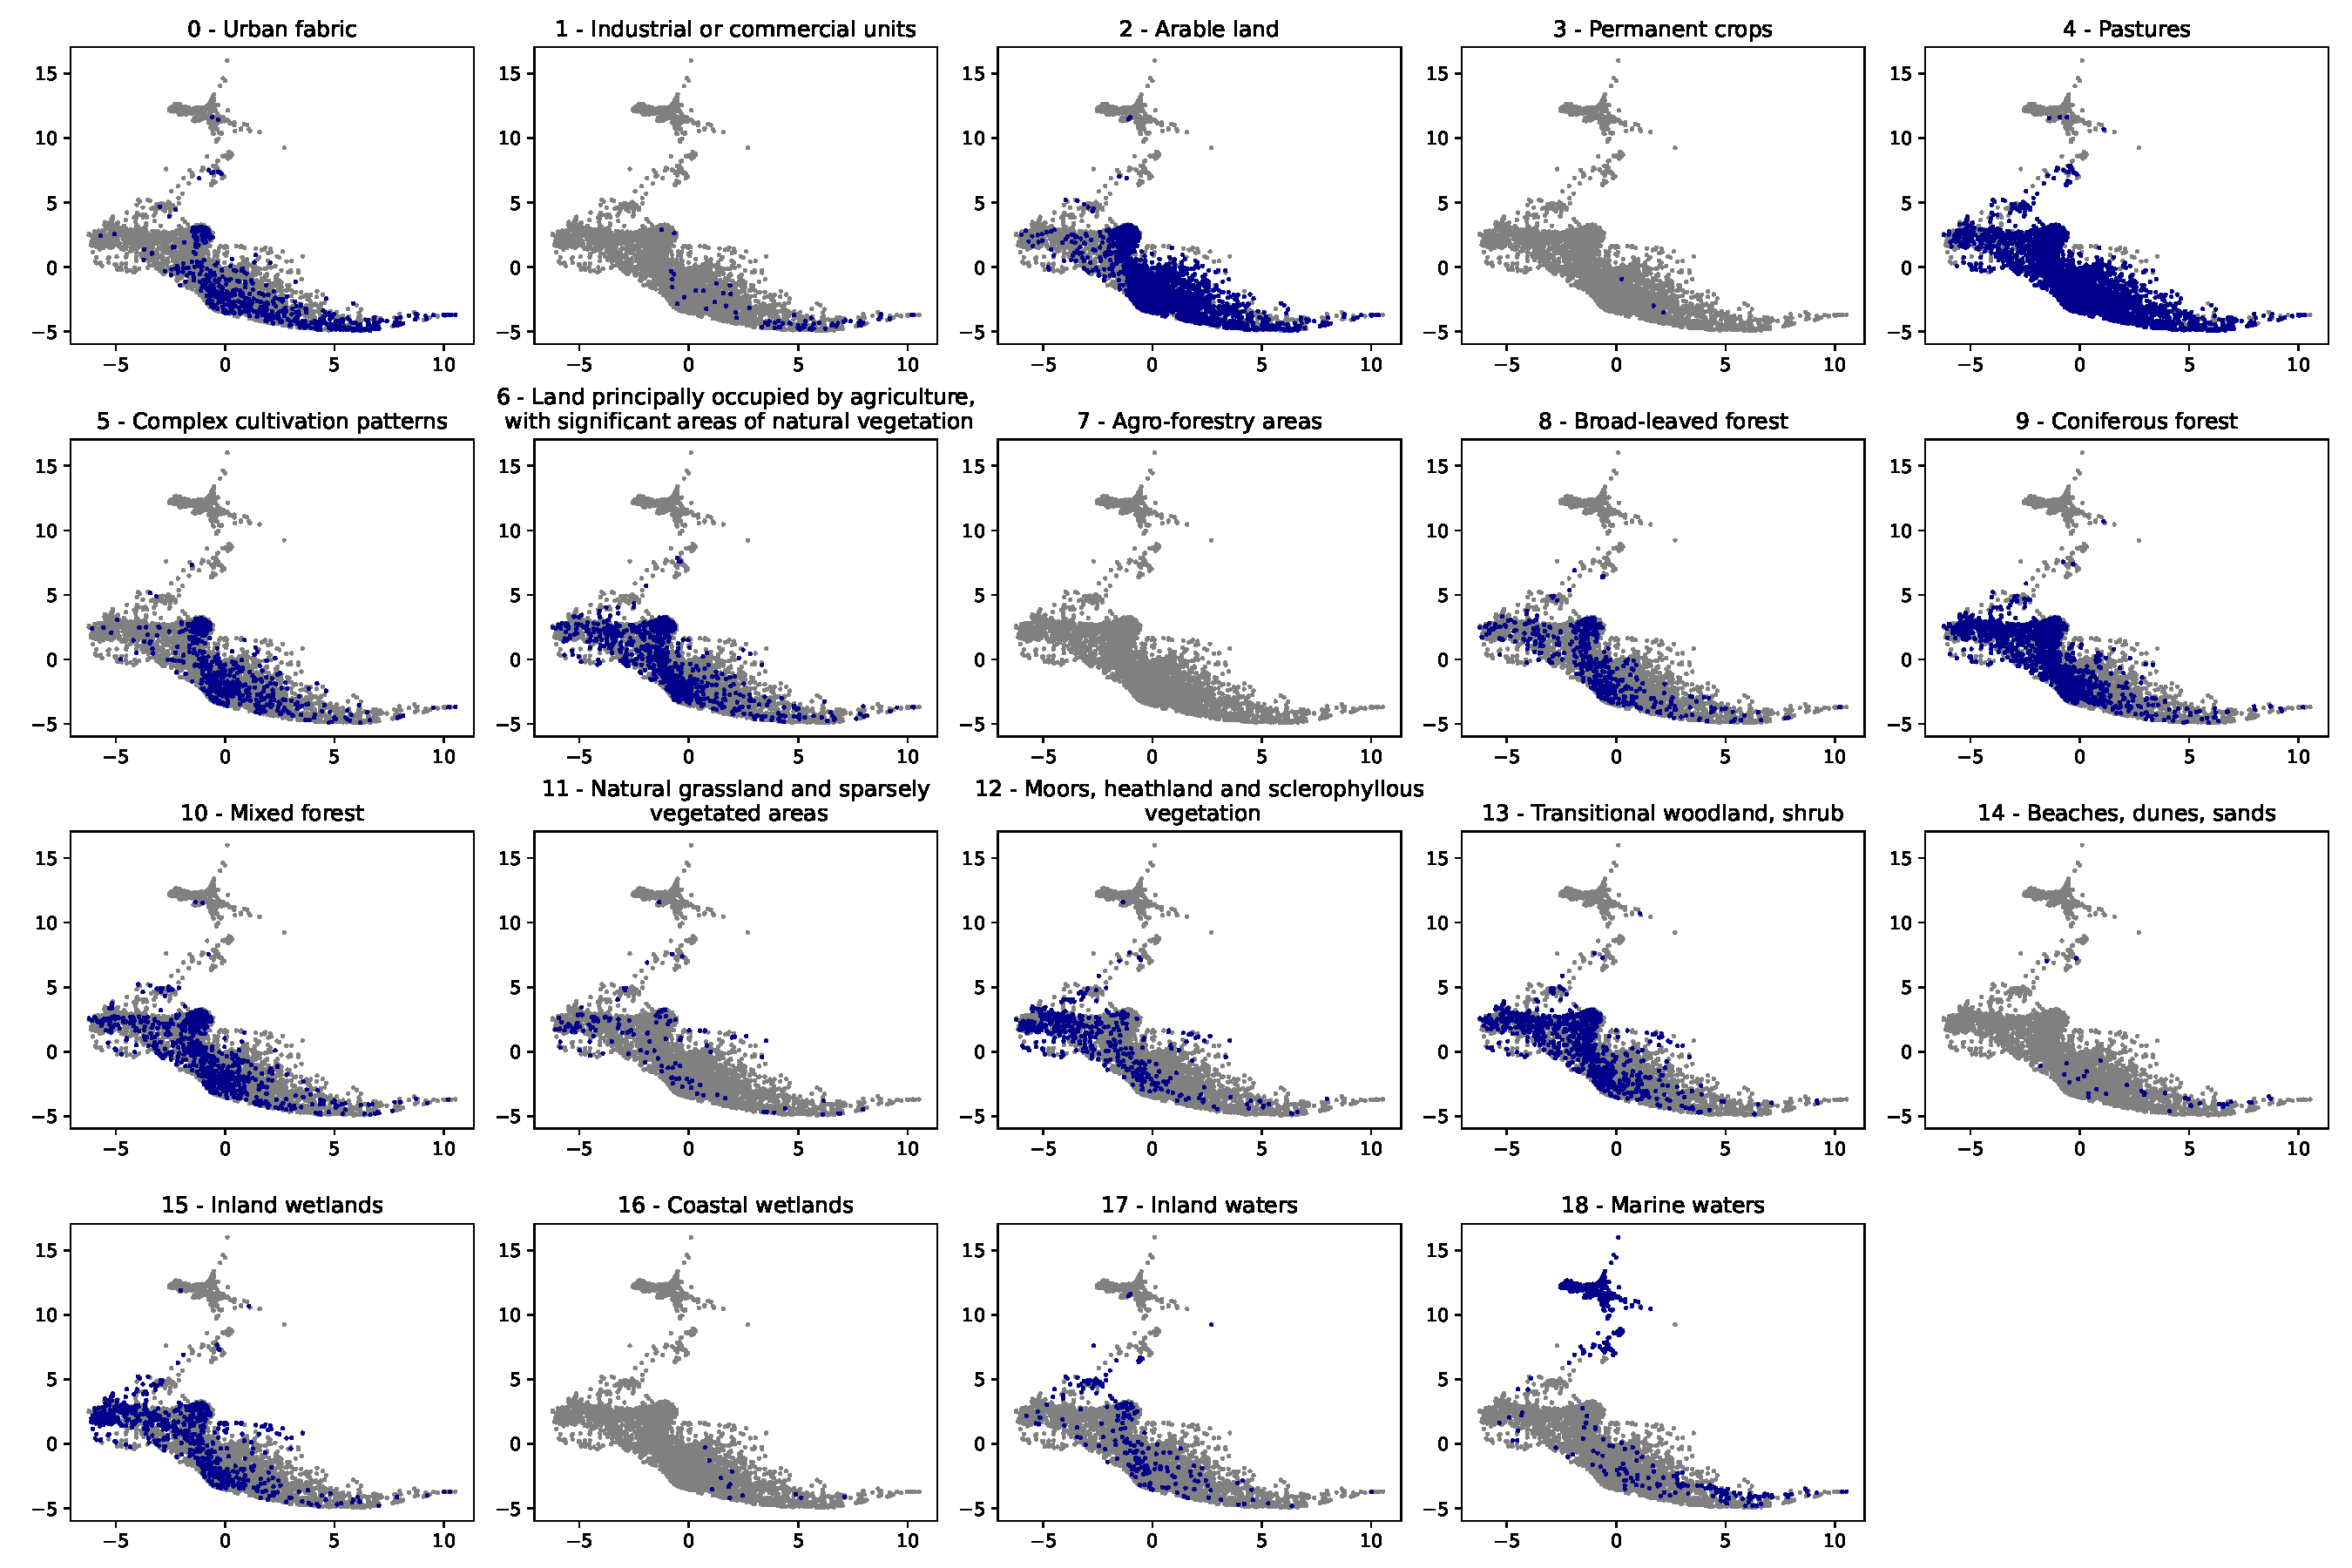
\includegraphics[width=\linewidth]{figures/all_labels_moco.pdf}
   %\captionsetup{justification=raggedleft, width=1.4\textwidth} #
   %\captionsetup{width=\linewidth} 
   %\vspace{2pt}
   \caption{MoCo-v2 foundation model.}
   \end{minipage}
\end{figure}

\begin{figure*}[htbp]
  \centering
   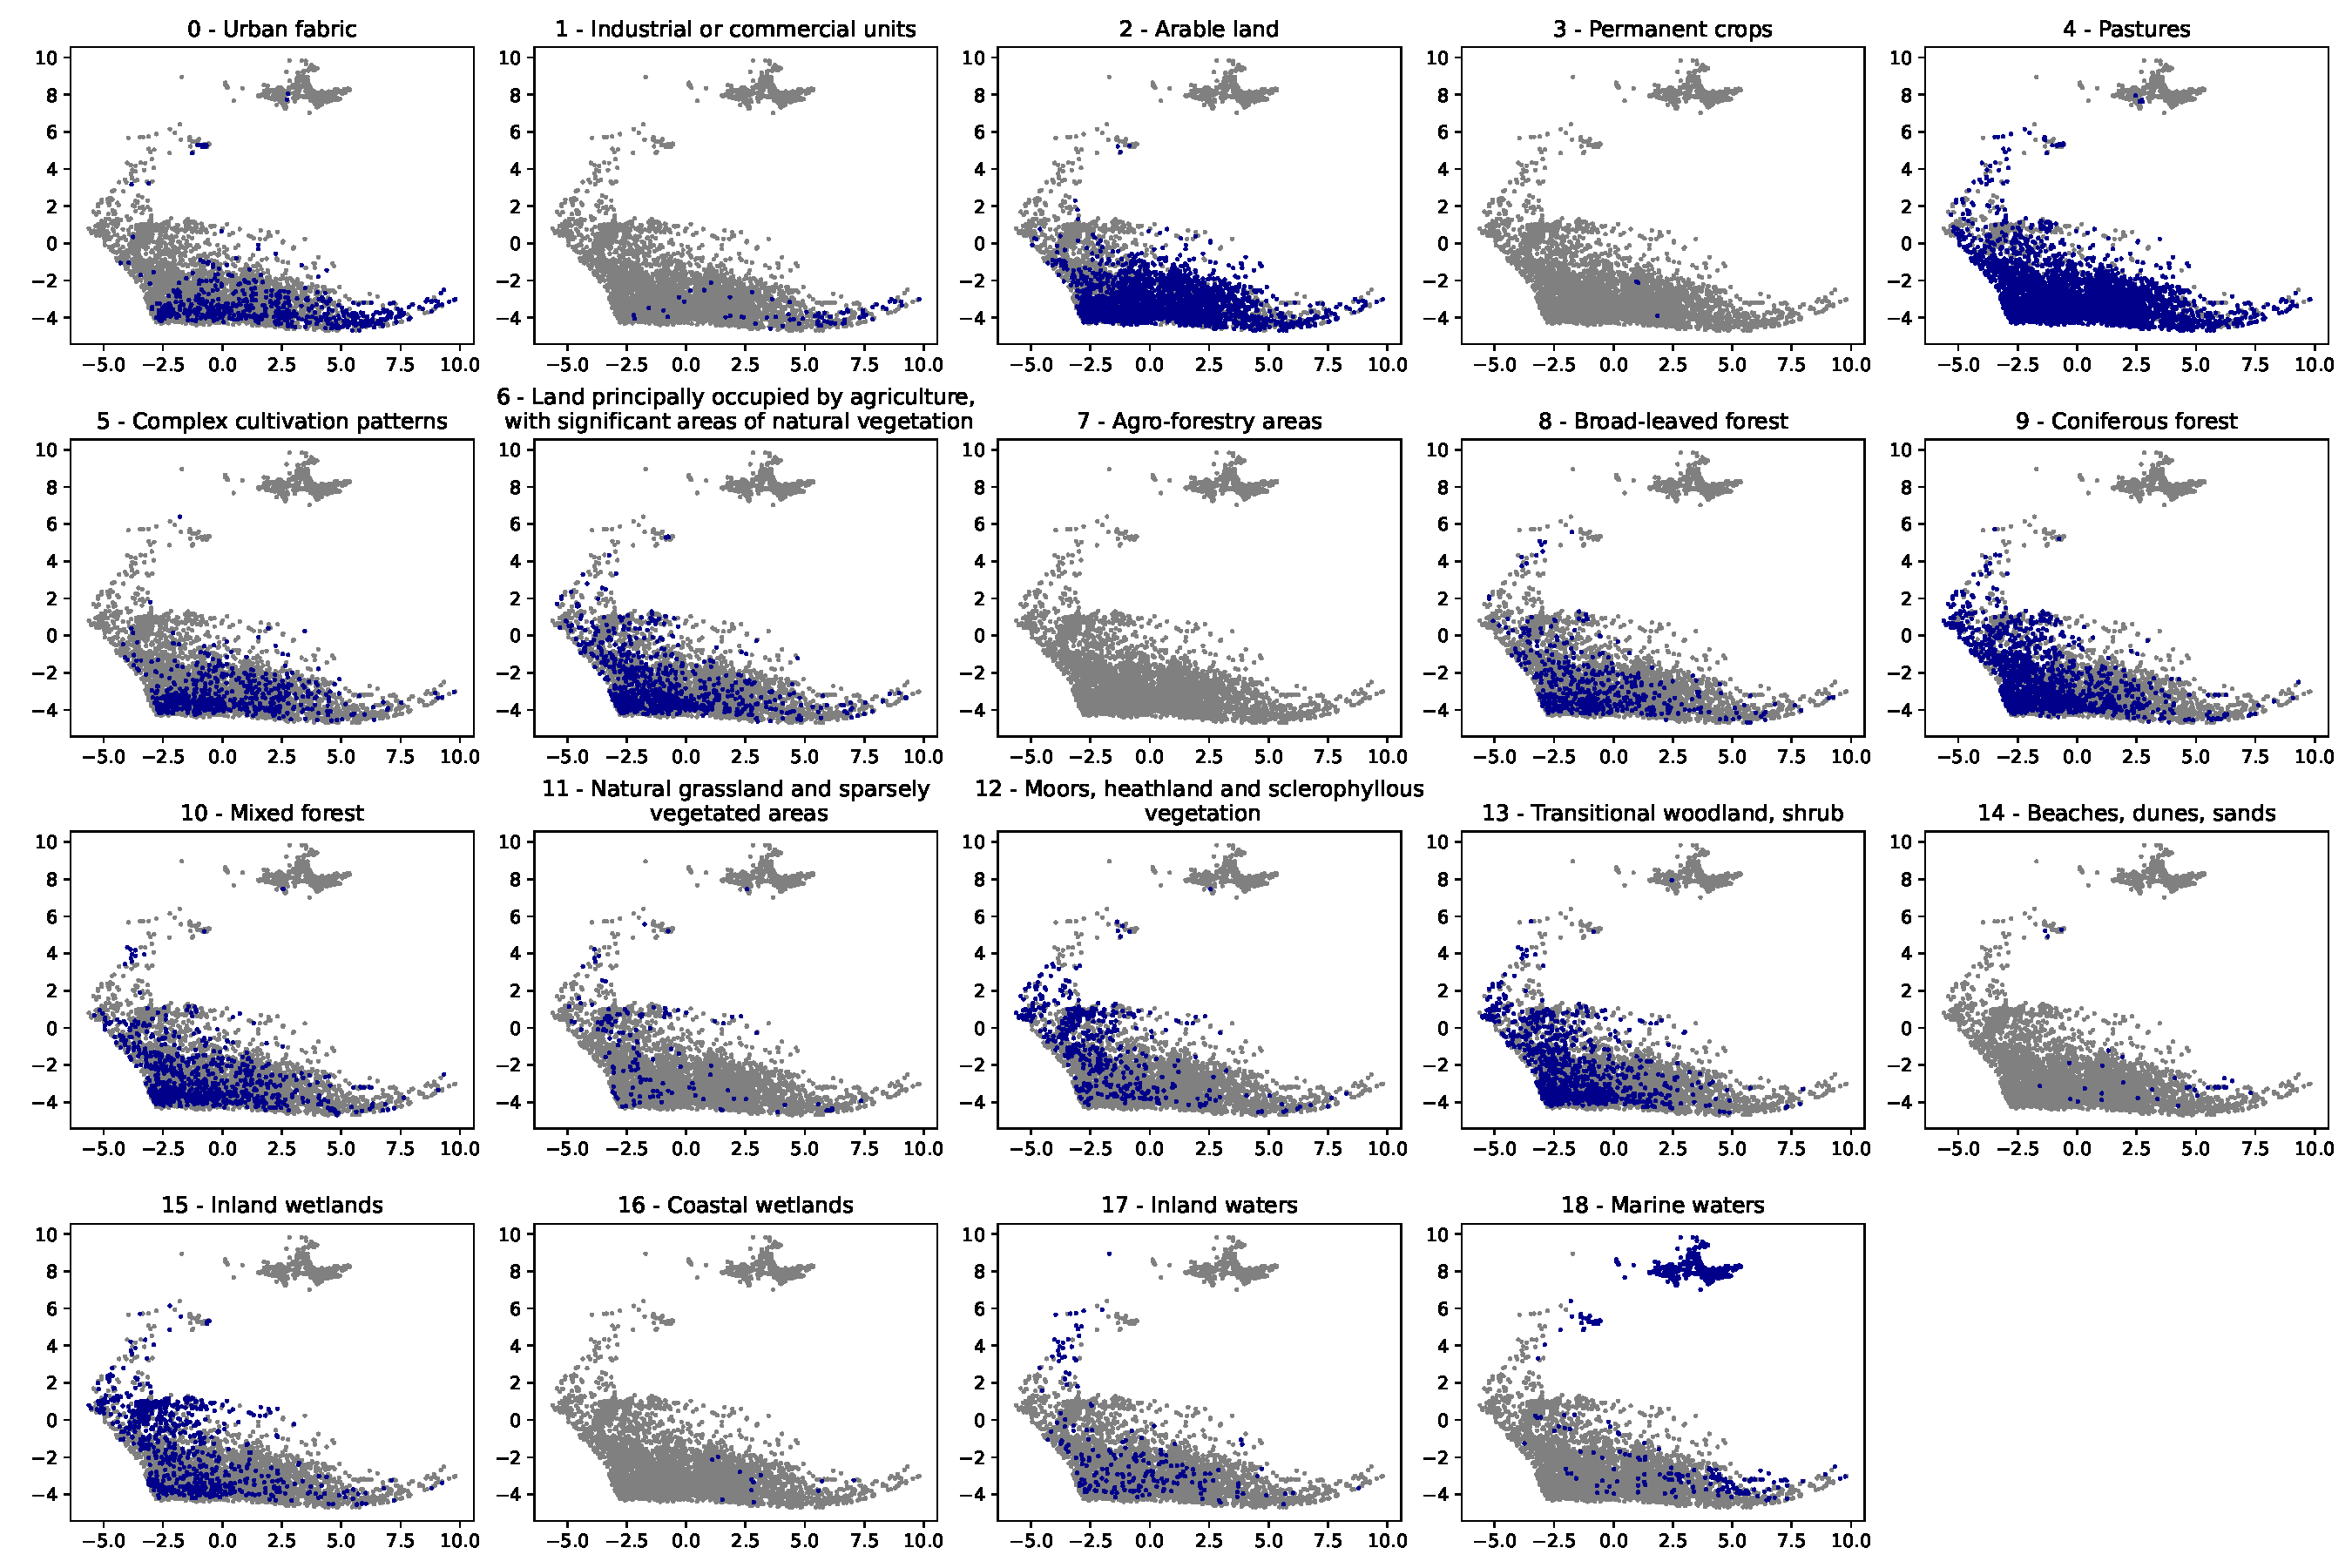
\includegraphics[width=\linewidth]{figures/all_labels_geo.pdf}
   \caption{MoCo-v2 additionally pre-trained on the geo-location classification task.}
\end{figure*}

\begin{figure*}[htbp]
  \centering
   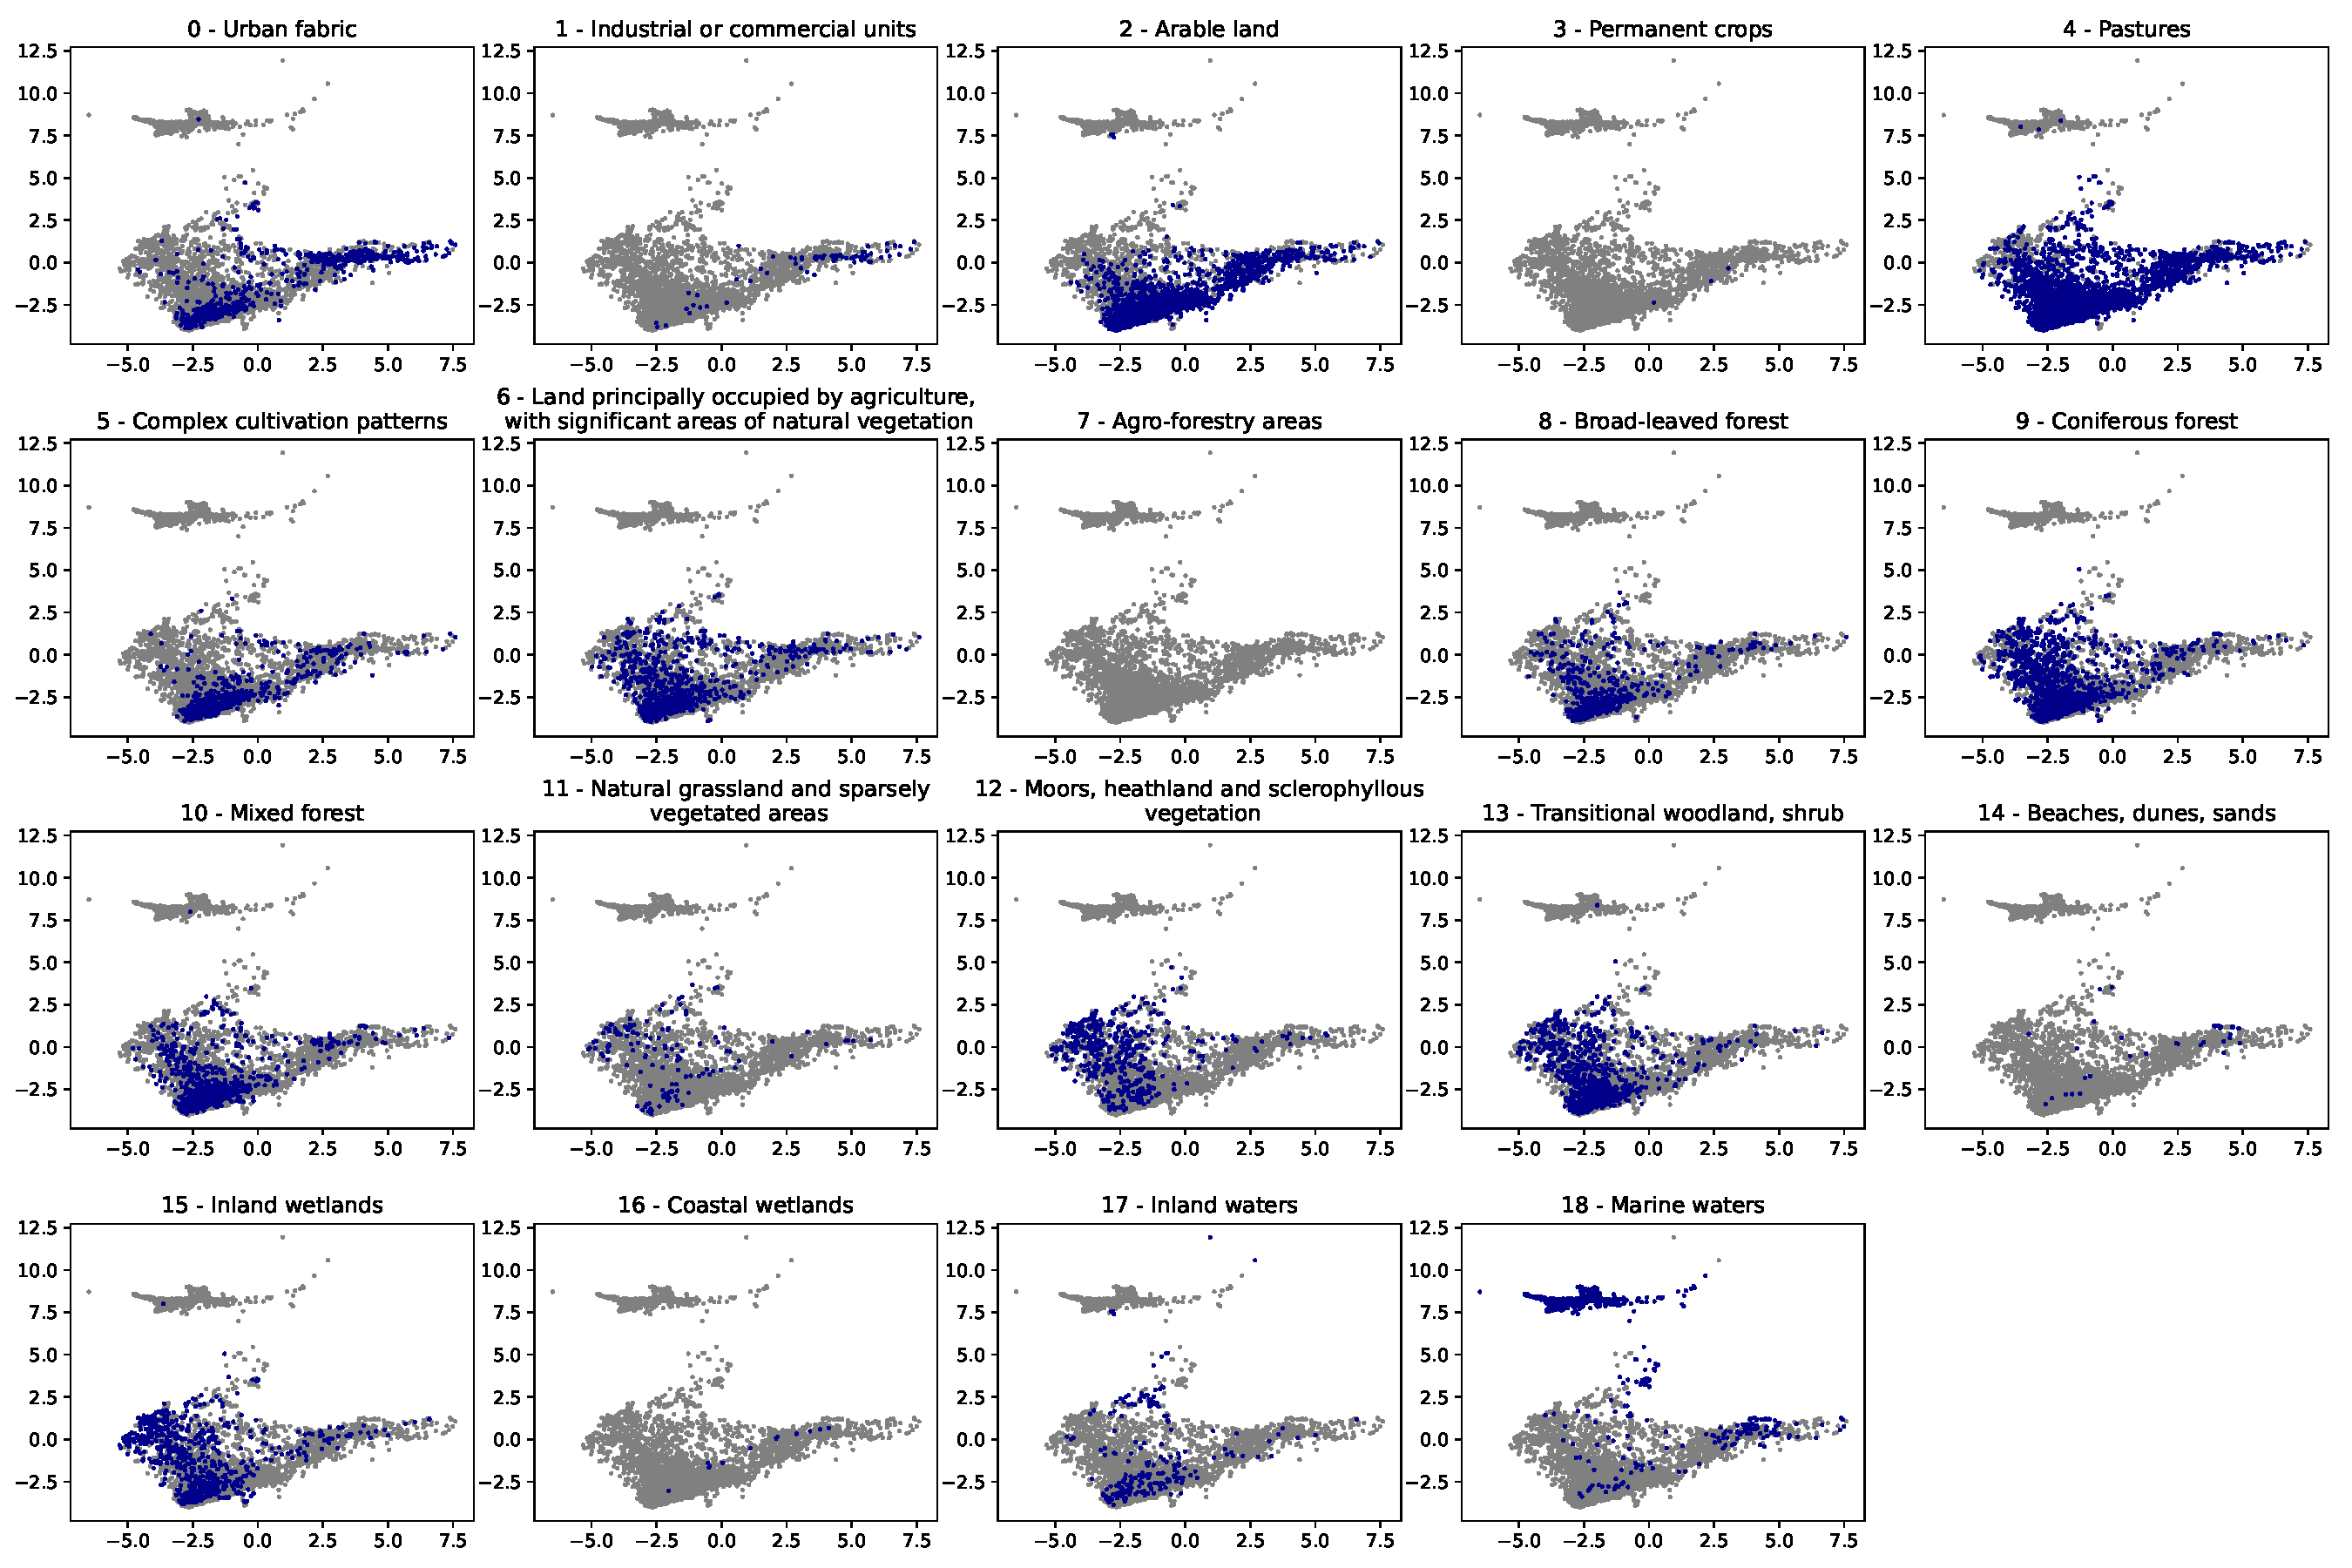
\includegraphics[width=\linewidth]{figures/all_labels_tp.pdf}
   \caption{MoCo-v2 trained with temporal positives.}
\end{figure*}

\begin{figure*}[htbp]
  \centering
   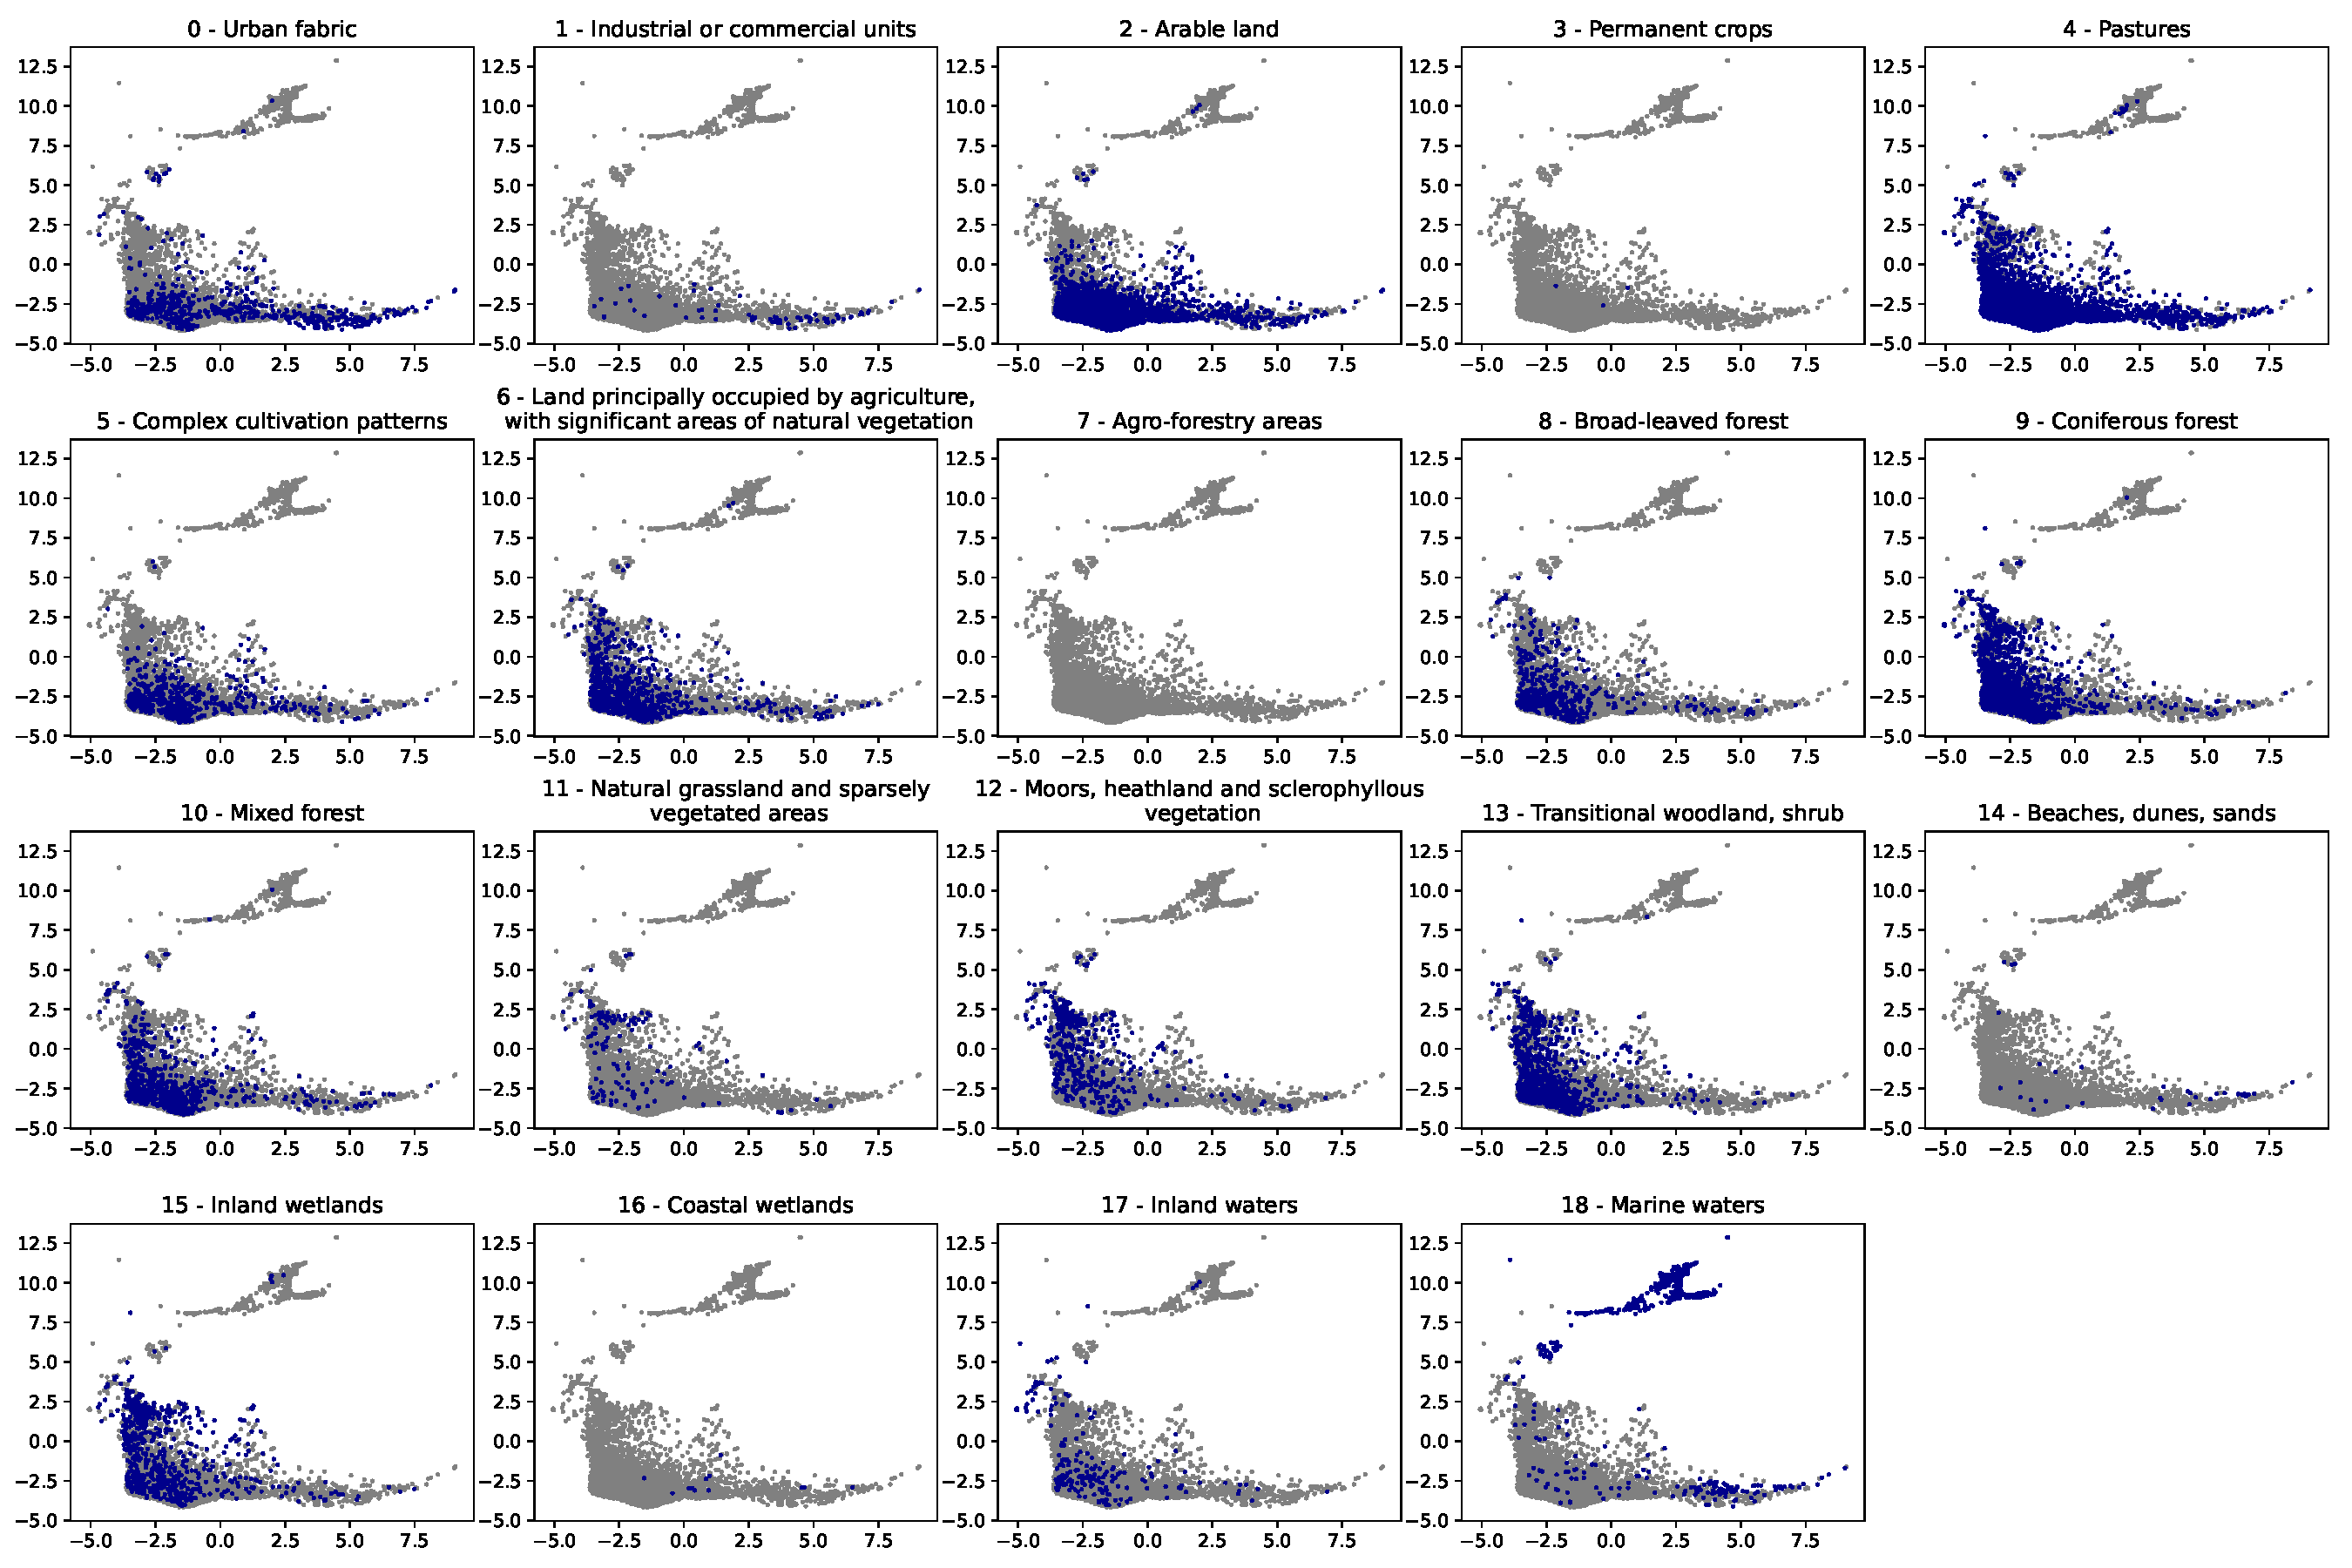
\includegraphics[width=\linewidth]{figures/all_labels_geo+tp.pdf}
   \caption{MoCo-v2 trained with temporal positives and on the geo-location classification task.}
\end{figure*}


% WARNING: do not forget to delete the supplementary pages from your submission 
% 
\clearpage
%\setcounter{page}{1}

\maketitlesupplementary

%\title{Reevaluation of Foundation Models in \\"Geography-Aware Self-Supervised Learning”}{Supplementary Material}
\section*{UMAP Feature Visualization} 

\vspace{10pt}
\begin{minipage}{\textwidth}
    The following figures visualize the UMAP features of the BigEarthNet-S2 test data's feature vectors extracted by the four re-evaluated foundation models.  The feature vectors that correspond to the specified class are shown in blue. This visualization is provided for each of the 19 labels. \\
\end{minipage}

\begin{figure}[htbp]
  \centering
   \begin{minipage}{\textwidth}
   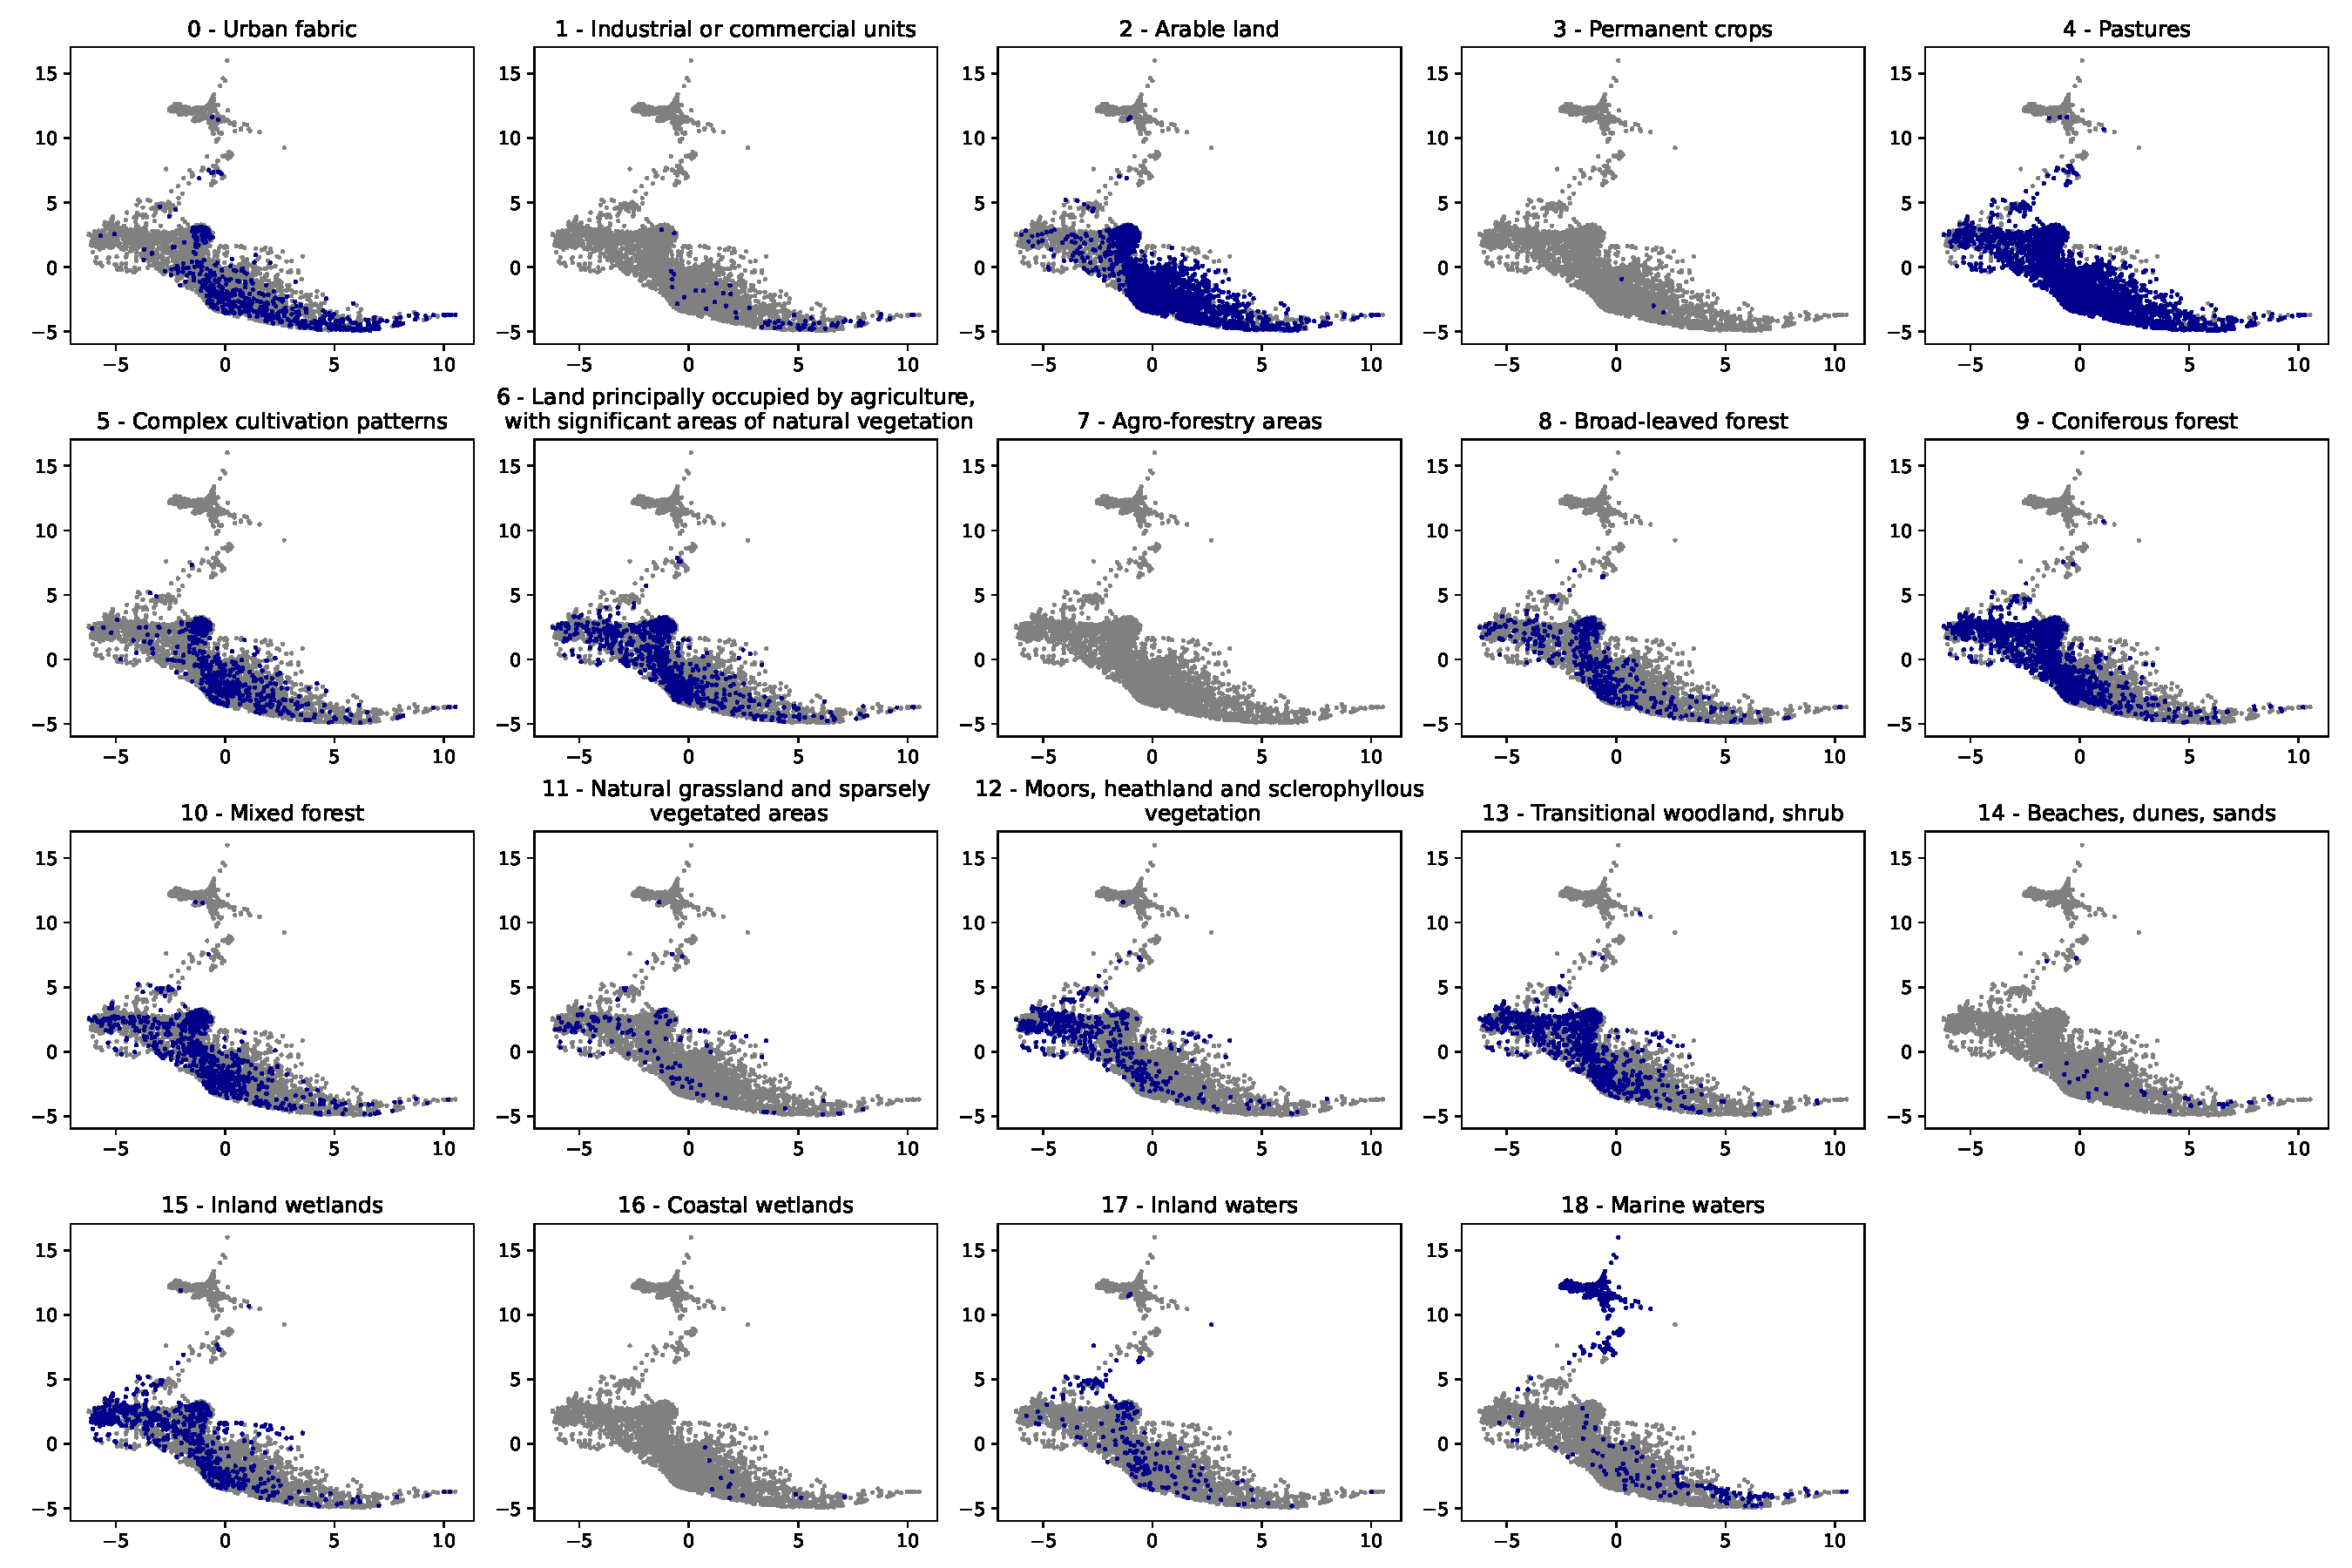
\includegraphics[width=\linewidth]{figures/all_labels_moco.pdf}
   %\captionsetup{justification=raggedleft, width=1.4\textwidth} #
   %\captionsetup{width=\linewidth} 
   %\vspace{2pt}
   \caption{MoCo-v2 foundation model.}
   \end{minipage}
\end{figure}

\begin{figure*}[htbp]
  \centering
   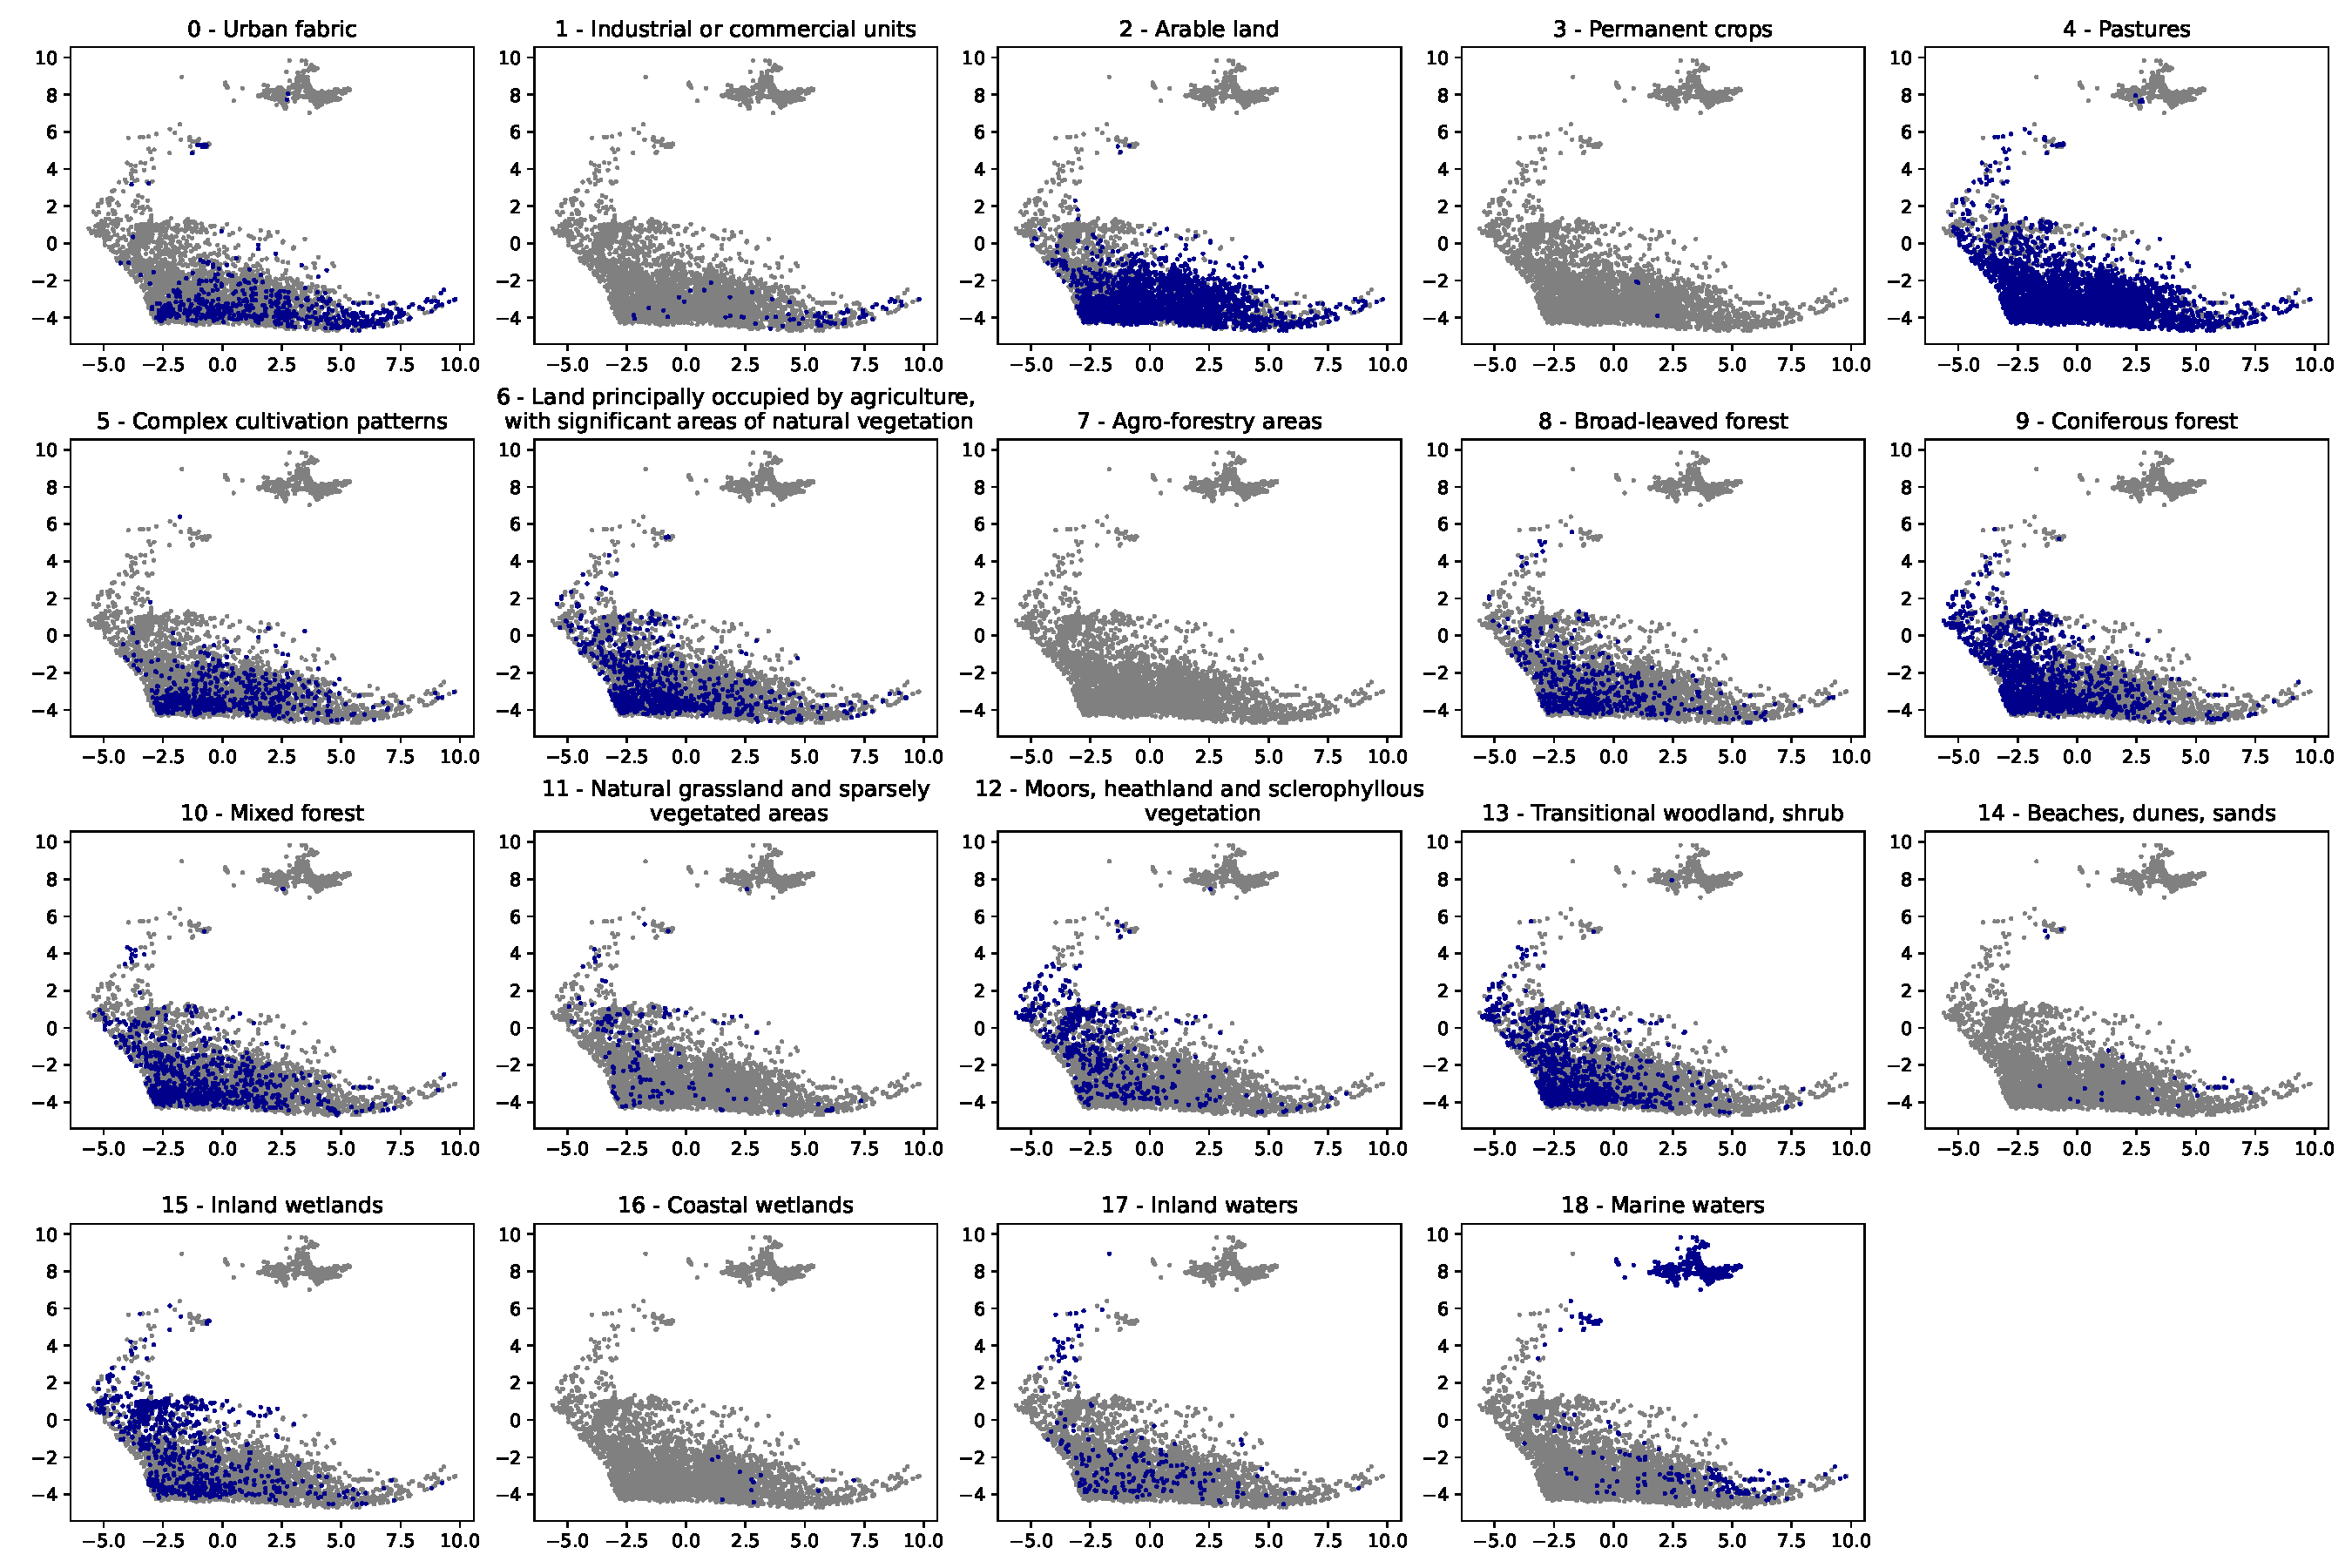
\includegraphics[width=\linewidth]{figures/all_labels_geo.pdf}
   \caption{MoCo-v2 additionally pre-trained on the geo-location classification task.}
\end{figure*}

\begin{figure*}[htbp]
  \centering
   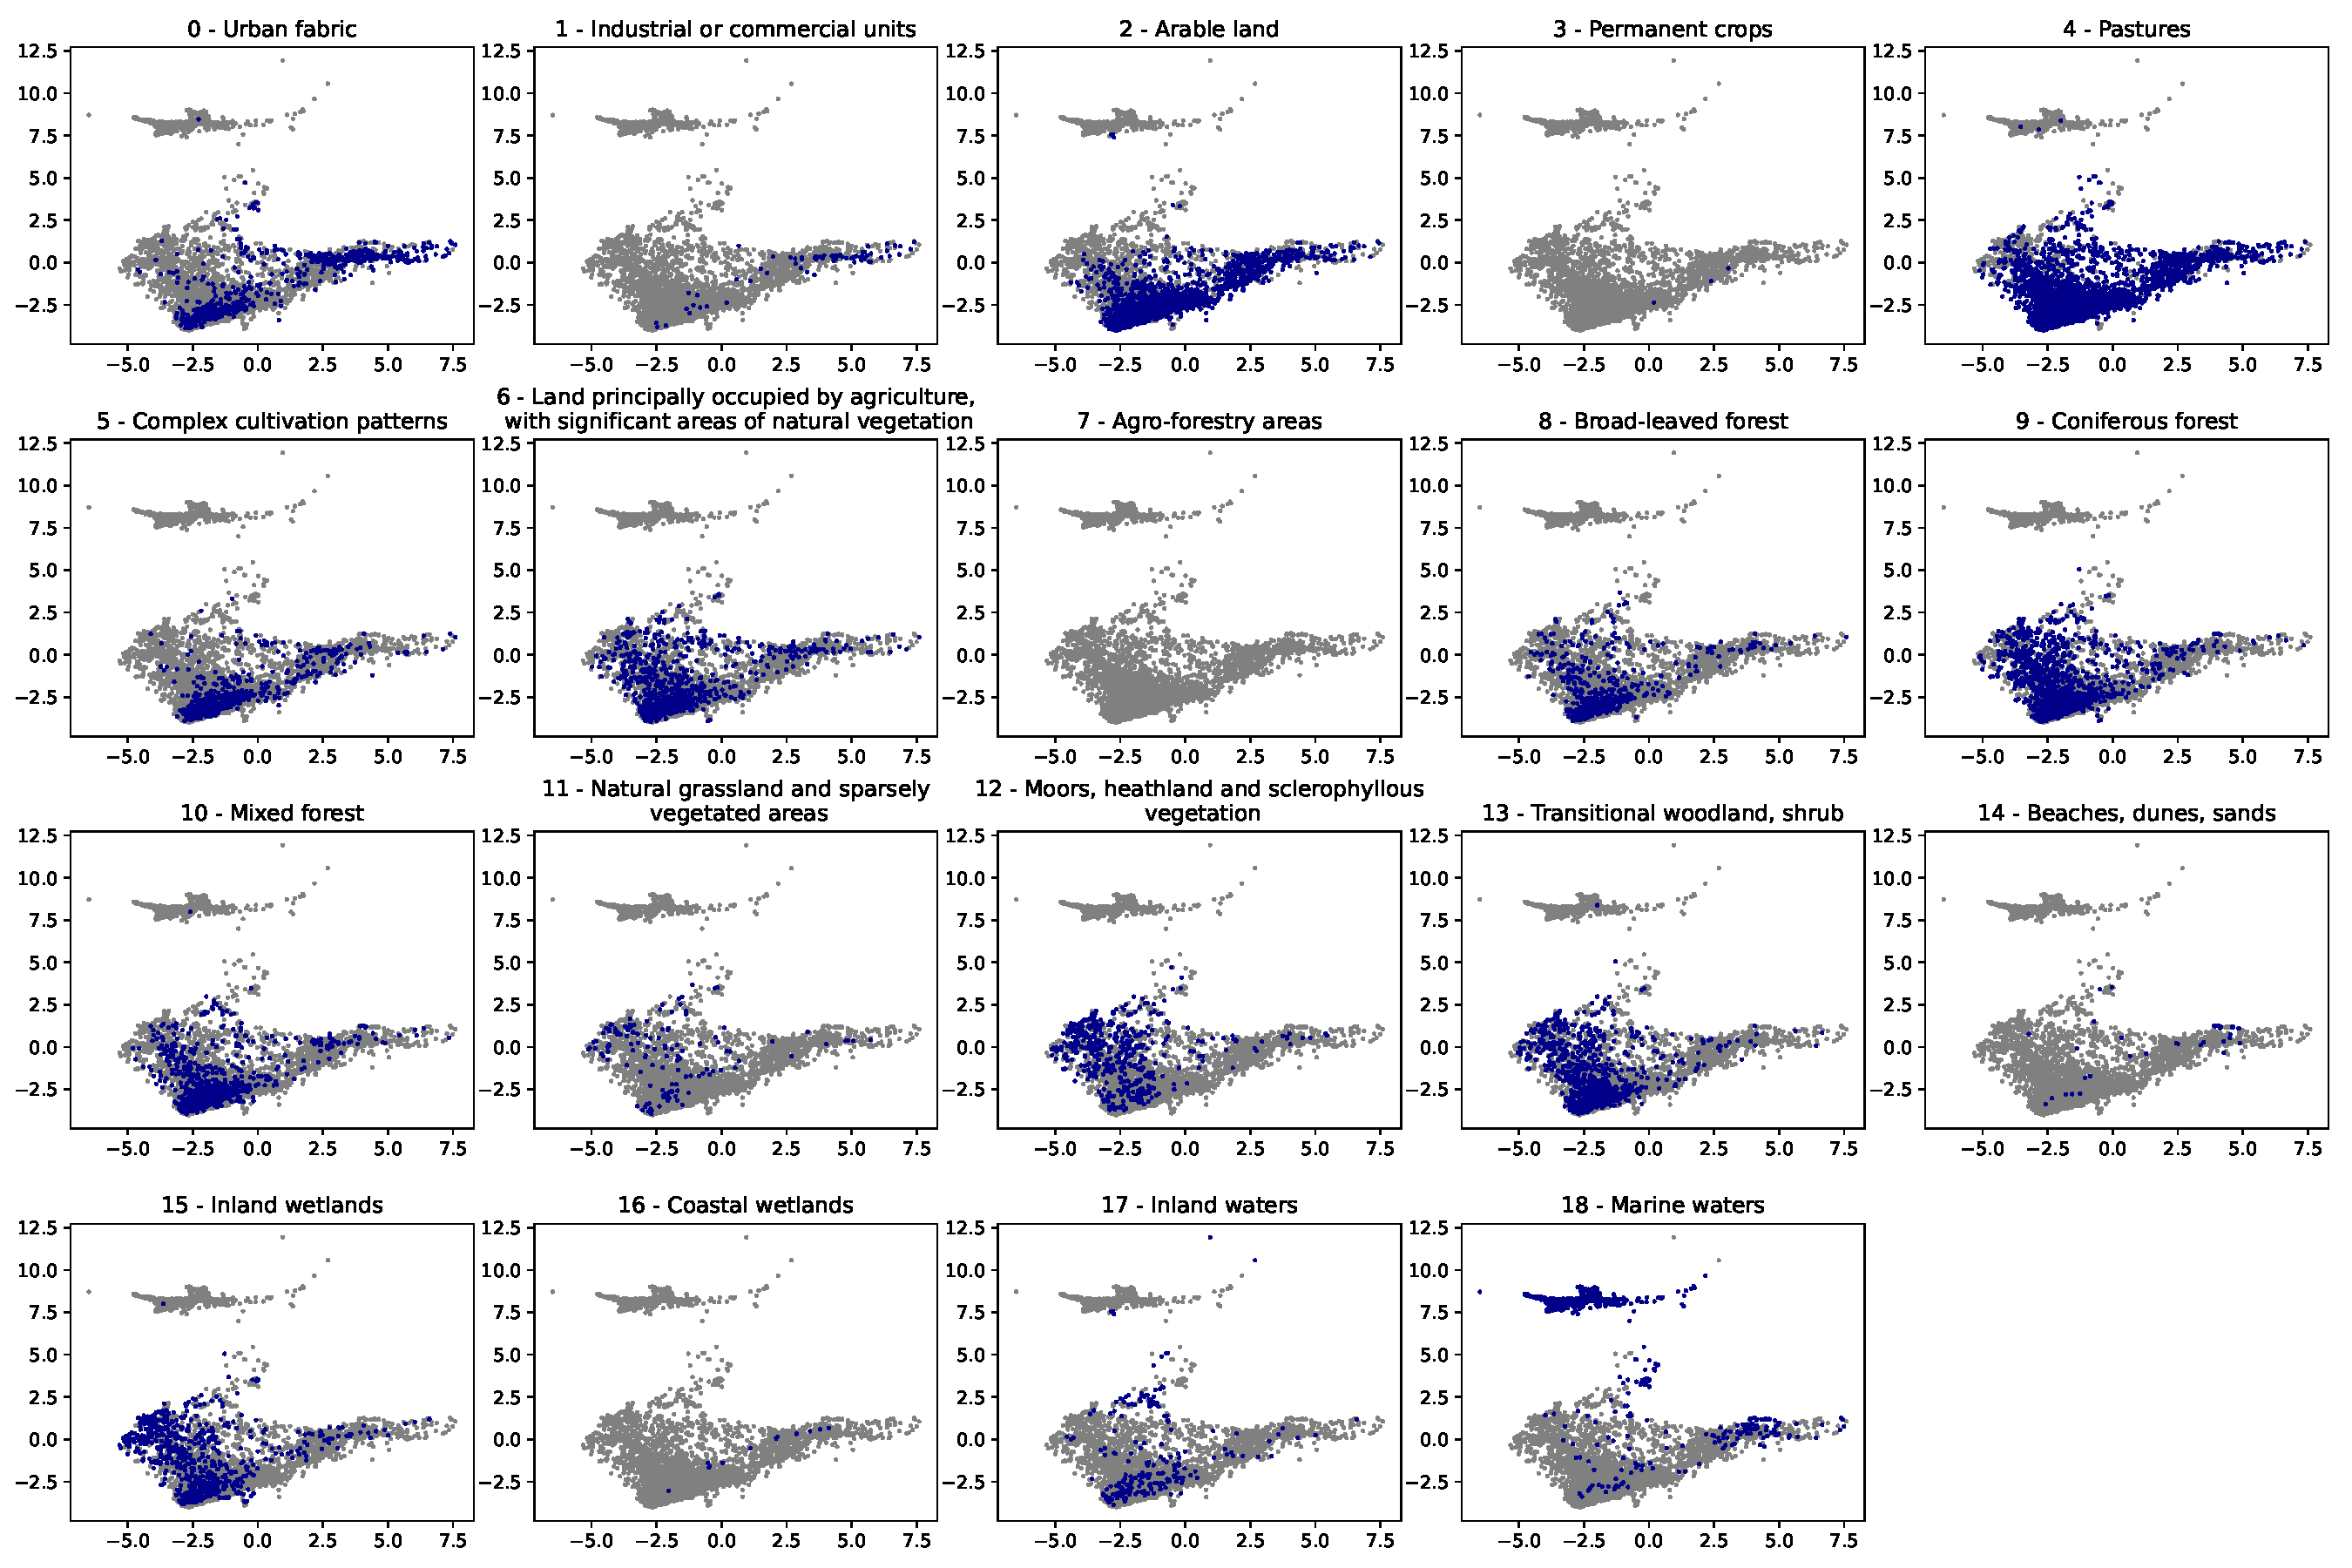
\includegraphics[width=\linewidth]{figures/all_labels_tp.pdf}
   \caption{MoCo-v2 trained with temporal positives.}
\end{figure*}

\begin{figure*}[htbp]
  \centering
   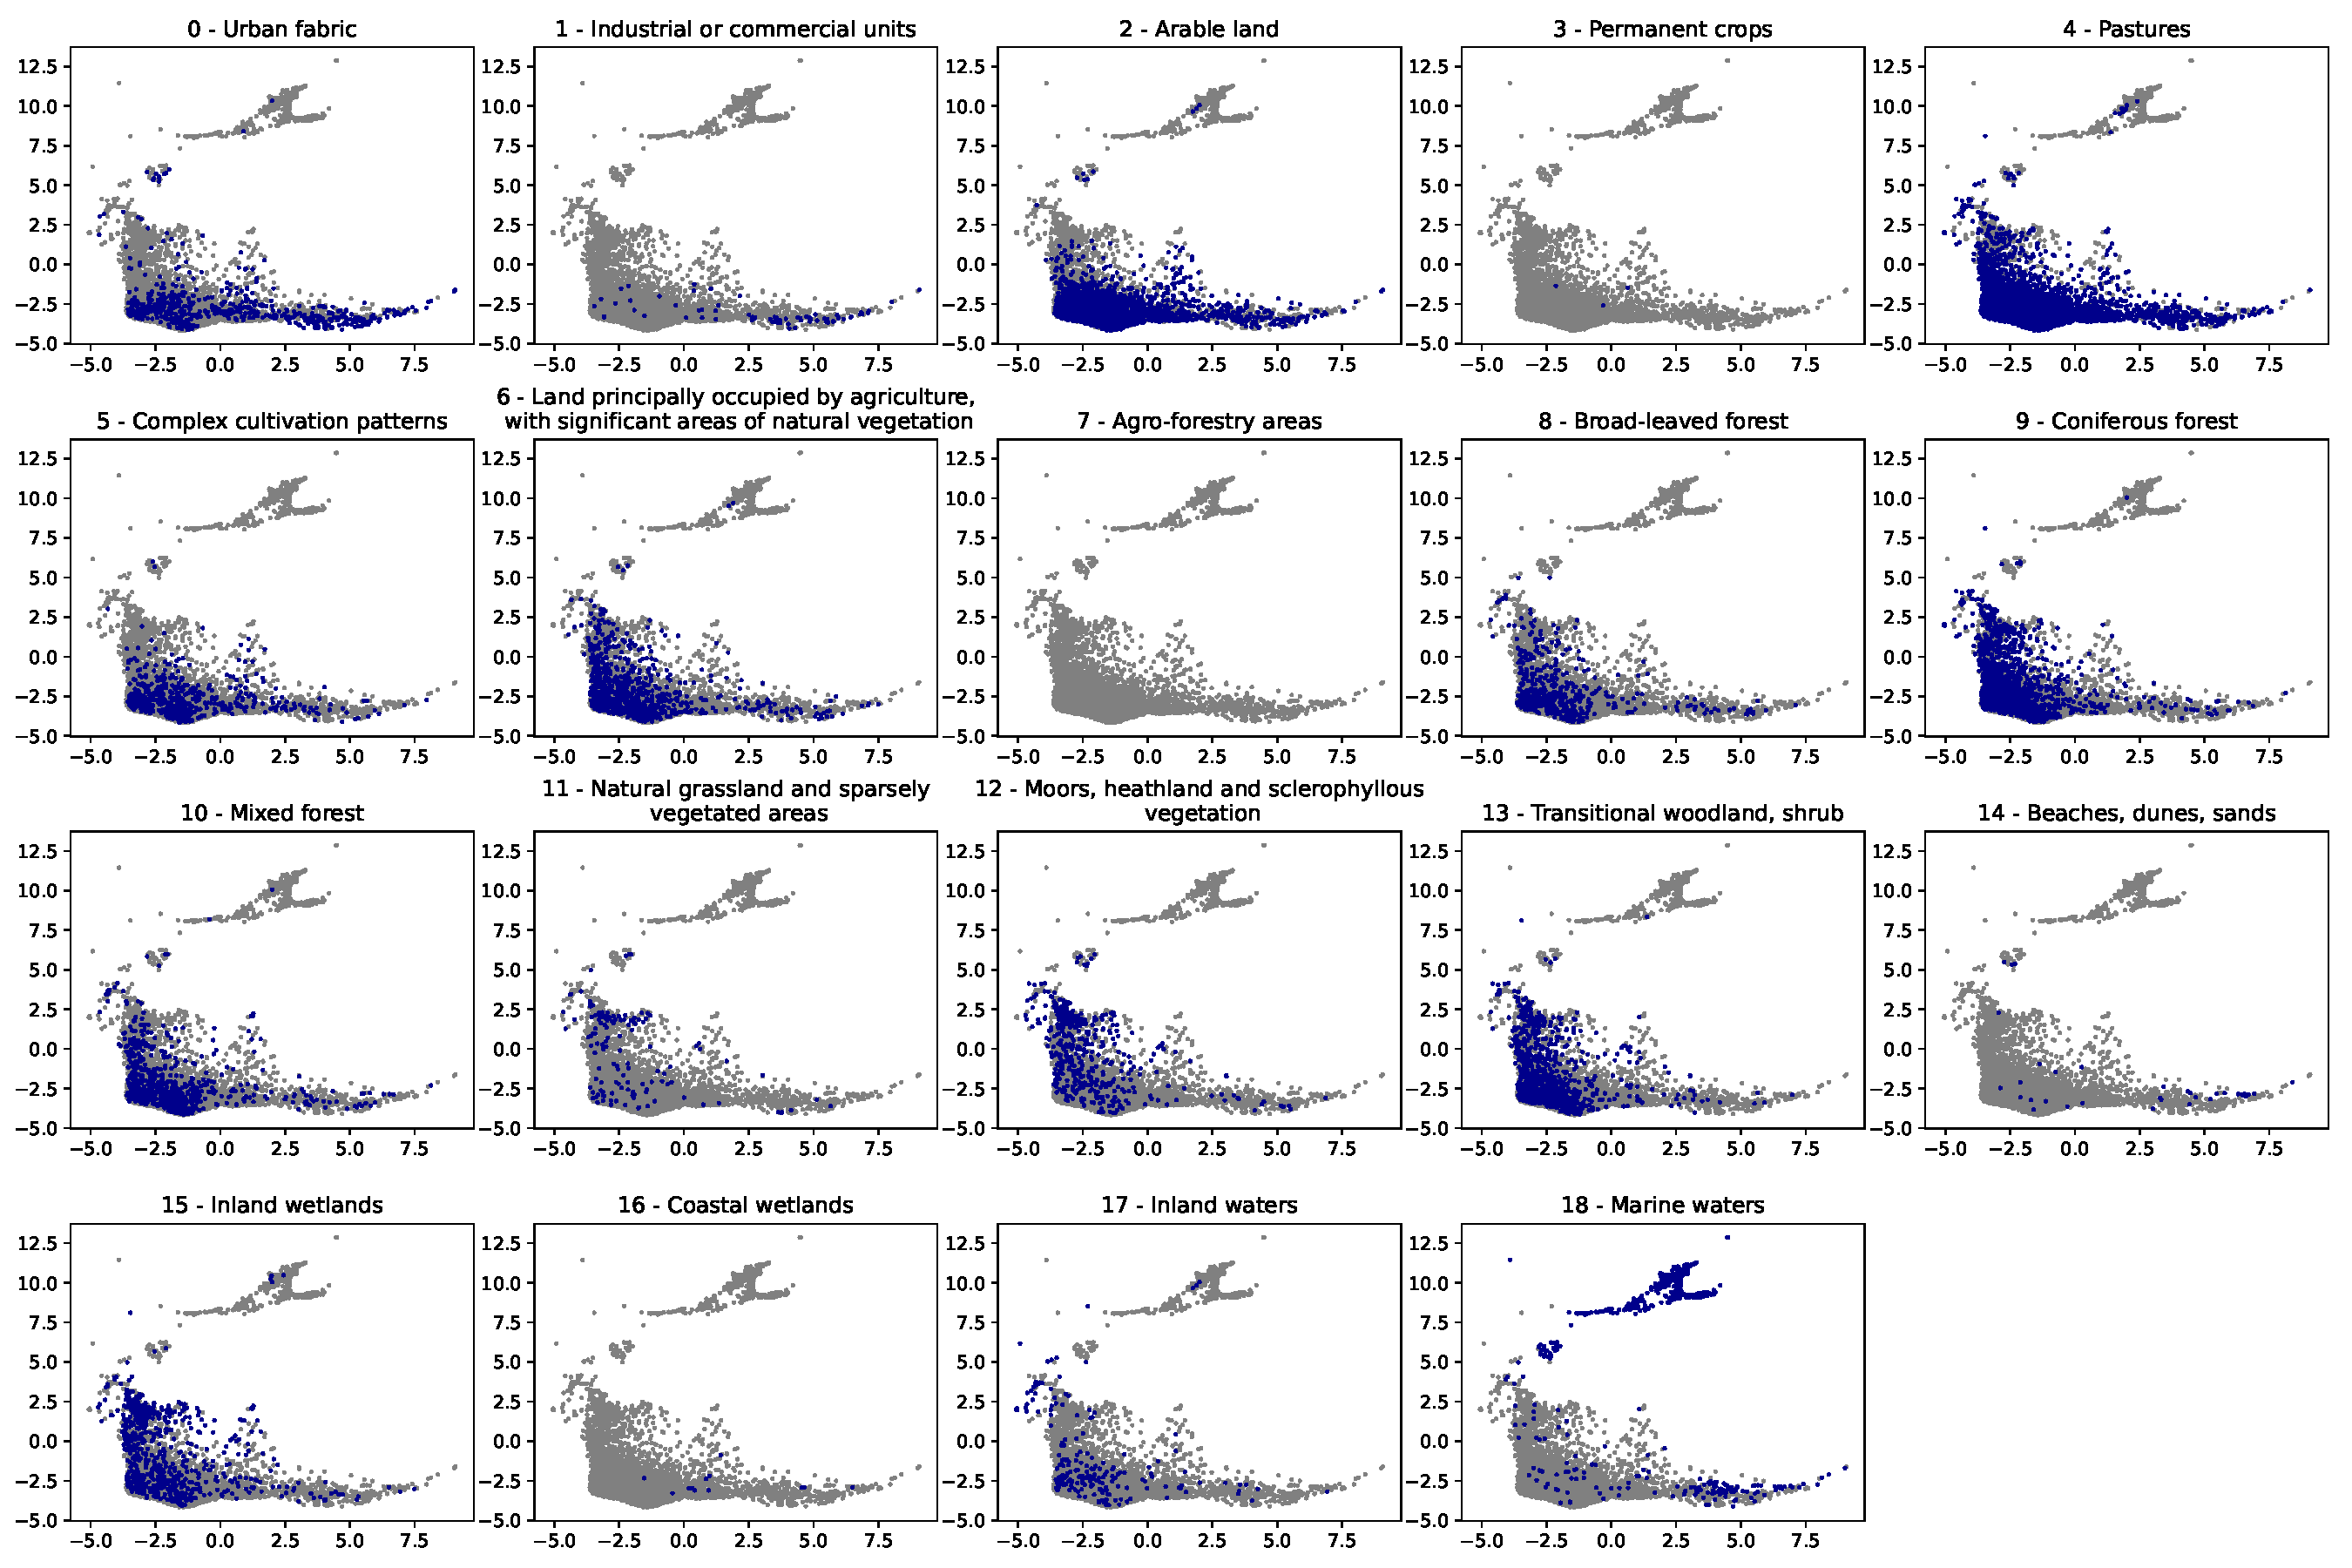
\includegraphics[width=\linewidth]{figures/all_labels_geo+tp.pdf}
   \caption{MoCo-v2 trained with temporal positives and on the geo-location classification task.}
\end{figure*}


\end{document}
